\documentclass[12pt]{article}
\usepackage{graphicx}
\usepackage[english]{babel}
\usepackage{listings}
\usepackage{color}
\usepackage{subcaption}
\usepackage{tikzscale}
\usepackage{mwe}
\usepackage{xcolor}
\usepackage{tabularx}
\usepackage{tabu}
\usepackage{mathtools}
\usepackage{wrapfig}
\usepackage{pdfpages}
\usepackage{physics}
\usepackage{amssymb}
\usepackage{pgfplots}
\usepackage{empheq}
\usepackage{float}
\usepackage[toc,section=section]{glossaries}
\usepackage[font={small,it}]{caption}
\usepackage{tikz}
\usetikzlibrary{decorations.pathreplacing}
\usetikzlibrary{3d}
\usepackage{cancel}
\newcommand{\myparagraph}[1]{\paragraph{#1}\mbox{}\\}
\usepackage{titlesec}
\usepackage[utf8]{inputenc}
\pagestyle{headings}
\newcommand{\doubleCross}{%
	\raisebox{-1pt}{%
		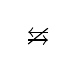
\begin{tikzpicture}w[scale = 3]%
		\draw [->] (0, 0) -- (0.25, 0);                 
		\draw [<-] (0, 0.1) -- (0.25, 0.1);     
		\draw [black](0.25,0.15) -- (0,-0.05);  
		\end{tikzpicture}
	}
}

\pgfplotsset{compat=1.16}

\newcommand{\singleCross}{%
	\raisebox{-1pt}{%
		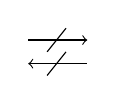
\begin{tikzpicture}[scale = 3]%
		\draw [<-] (0, 0) -- (0.25, 0);            
		\draw [black](0.16,0.15) -- (0.08,0.05);   
		\draw [->] (0, 0.1) -- (0.25, 0.1);       
		\draw [black](0.16,0.05) -- (0.08,-0.05);   
		\end{tikzpicture}
	}
}

% Add linebreaks to very long urls (otherwise it's off-site)
\usepackage{url}
\makeatletter
\g@addto@macro{\UrlBreaks}{\UrlOrds}
\makeatother

% Hyperlinks in contents
\usepackage{hyperref}
\hypersetup{
    colorlinks,
    citecolor=black,
    filecolor=black,
    linkcolor=black,
    urlcolor=black
}
% Make links look great again
\urlstyle{same}

% Silence hyperref warnings about math formulas in sections, make sure to include new characters used
\pdfstringdefDisableCommands{%
%  \def${}%
  \def\alpha{alpha}%
  \def\epsilon{epsilon}%
  \def\gamma{gamma}%
  \def\({}%
  \def\){}%
  \def\texttt#1{<#1>}%
}

% Glossary settings
% Set first occurency to italics 
\defglsentryfmt{%
  \ifglsused{\glslabel}{%
    \glsgenentryfmt%
  }{%
    % Typeset first use
    \textit{\glsgenentryfmt}%
  }%
}
\makeglossaries
\loadglsentries{glossaries}
\glsenablehyper
\glsresetall

\begin{document}

\definecolor{dkgreen}{rgb}{0,0.6,0}
\definecolor{gray}{rgb}{0.5,0.5,0.5}
\definecolor{mauve}{rgb}{0.58,0,0.82}
\definecolor{backcolour}{rgb}{0.95,0.95,0.92}
\definecolor{gray}{rgb}{0.4,0.4,0.4}
\definecolor{darkblue}{rgb}{0.0,0.0,0.6}
\definecolor{cyan}{rgb}{0.0,0.6,0.6}
\definecolor{brightcerulean}{rgb}{0.11, 0.67, 0.84}

\lstset{frame=tb,
  backgroundcolor=\color{backcolour},   
  aboveskip=3mm,
  belowskip=3mm,
  showstringspaces=false,
  columns=flexible,
  basicstyle={\small\ttfamily},
  numbers=none,
  numberstyle=\tiny\color{gray},
  keywordstyle=\color{blue},
  commentstyle=\color{dkgreen},
  stringstyle=\color{mauve},
  breaklines=true,
  breakatwhitespace=true,
  tabsize=3
}
\begin{titlepage}
    \centering
    \includegraphics[width=1\textwidth]{pictures/title.pdf}\par\vspace{0.5cm}
    {\scshape\LARGE Kantonsschule Wohlen \par}
    \vspace{0.2cm}
    {\scshape\Large Matura-project\par}
    \vspace{2cm}
    {\huge\bfseries Creating an AI which can play games\par}
    \vspace{2cm}
    {\Large\itshape Brian Funk and Silvan Metzker\par}
    \vfill
    supervised by\par
    Patric \textsc{Rousselot} and Mark \textsc{Heinz}
    \vfill 
    {26. Oktober, 2020}
\end{titlepage}
\tableofcontents
\newpage
\section{Abstract}
The term \gls{artificial intelligence} (\gls{AI}) is widely used. Many know this wording in the context of a science fiction movie or when it comes to data analysis. Google uses \gls{AI} to provide their customers with the optimal advertisement. It works, but hardly anyone can imagine how it works. By programming and testing such an intelligence, we try to understand how exactly this can work. How well can an \gls{AI} perform the tasks given? Where will we face limitations? These and many other questions are answered in this report. \\
We succeeded in implementing an \gls{AI} in various games. But it doesn't work equally well for all of them. We encountered the limits of intelligent retrieval sooner than we thought. But one of the goals of this project is to simply understand the technology. Even though the products are not perfect, we gained a lot of knowledge and thus achieved our main goal.
\section{Introduction}
The goal of this project is to create an \gls{AI} that can play games. This is achieved by utilizing a practice called \gls{machine learning}. \Gls{machine learning} is defined as a technique that can learn by using \gls{computational power}. It's a generic term mainly used to describe \gls{AI}s which learn by analyzing huge amounts of data. 
The most human-like strategy in \gls{machine learning} is \gls{deep learning}. It's structure is similar to a human brain and does surprisingly well at mimicking the brain's abilities to learn. \\
This report is structured in the same way, we encountered the problems. First, the theoretical foundation has to be laid out. This will be done in chapter \ref{basics}. To make it more tangible, this theoretical part will be backed up by a real-life example. There are many different ways to perform \gls{machine learning}. Those range from just taking values out of a table, to a methodology similar to a human brain. To decide which type of \gls{machine learning} to use, a clear difference has to be made. This will be discussed in chapter \ref{reinflear}. As soon as it was clear, which type will be used, it had to be implemented. How this exactly happened, is stated in the implementation chapter. To gain some insights, the subsequent chapter shows some basic coding. \clearpage The whole project can now be split into three parts: 

\begin{itemize}
    \item \Gls{artificial intelligence}
    \item Graphics
    \item Games
\end{itemize}
Each part will be discussed in chapters \ref{sec:TheModel}, \ref{GUI} and \ref{sec:Games}. What this implementation yields and how it performs with each game is recorded in chapter \ref{sec:results}. The games are increasingly complex, to test the capability of handling complex information.
\section{Basics of Artificial Neuronal Intelligence}\label{basics}
The upcoming section will explain, what is necessary in order to understand how an AI works. The first part will show what types of AI there are and which is being used in this project. The second part will explain in detail, how the mathematics behind neuronal networks work.
\subsection{What is an Artificial Intelligence?}
An \gls{AI} is the ability of a digital device to execute tasks, which are related to human beings and animals. This vague description can be taken in many ways, so a closer description would be an \gls{artificial narrow intelligence}. \cite{aibritannica}\\
\Gls{artificial narrow intelligence} (ANI) is a type of \gls{AI}, which can only be applied to one narrow task. This is the kind of \gls{AI} that currently exists. It can do a task very well, even better than humans. For example an \gls{AI}, can detect brain tumors way more accurately than an experienced neurosurgeon is expected to do. It's revolutionary and does very well at one certain task, however, it cannot tell the difference between a cat and a dog. This is considered an \gls{artificial narrow intelligence}. An \gls{artificial general intelligence} (AGI) on the other hand, is an \gls{AI} that can perform all tasks that a human can fulfill. This type of \gls{AI} is not yet discovered. The step after this, would be an \gls{artificial super intelligence} (ASI), this is the kind of \gls{AI} that is superior in every way to a human. It's also considered as the type of \gls{AI} which could lead to the extinction of the human race. The closest approach to one of those higher levels of an \gls{AI} was achieved by one of the so-called artificial \glspl{neuronal network} (\glspl{ANN}).
\cite{narrowAI} 
\subsection{Mathematics Behind an Artificial Neuronal Network}
This chapter will explain in detail how neuronal networks mathematically function. This basic knowledge is important if one wants to understand the outputs of a \gls{neuronal network} and how they are computed.
\subsubsection{Neuronal Network}\label{sec:nnmath}
A model that is used for many self-learning applications is called artificial \gls{neuronal network} or just  \gls{neuronal network}. This model mimics the human brain and tries to describe the learning-behaviour as accurately as possible. Although it has biological foundations, it can be described in a purely mathematical way. To understand this, certain terms have to be defined mathematically and linguistically.
Similarly to the brain, a \gls{neuron} takes multiple  \glspl{input} and passes an output forward, which is somehow dependant on the  \gls{input}. The human brain uses an electrical currents to transfer information. The \gls{AI} does this numerically. So a number gets passed from one neuron to another. The \glspl{input} of a \gls{neuron} are multiplied by a certain factor. Later in the learning process, these factors are the values, that are going to be optimized and changed. By increasing or decreasing these values, one node can either have more or less impact. If a junction has the \gls{weight} of $0$, the incoming number doesn't affect the network at all. The \gls{neuron} takes all the \glspl{input} and adds them together. This sum gets forwarded to the \gls{activation function}, which calculates the value according to the function. This transformed value gets forwarded to the next neuron and the whole process starts again. Two \glspl{neuron} can make a connection, which is used to pass the numerical \glspl{output} of the function to the next neuron. These \glspl{neuron} build up \glspl{layer} and determine its size by the amount of \glspl{neuron}. One of the properties of the  \glspl{layer} is, that all \glspl{neuron} from one \gls{layer} don't connect to each other. But they do connect to the previous and subsequent \glspl{layer}. The \glspl{layer} can be categorized in three different ways:  \gls{input}, output and \glspl{hidden layer}. The hidden \glspl{layer} describe all \glspl{layer}, except the in- and \glspl{output layer}. \cite{neuronal_network}\\
\begin{figure}[ht]
\begin{center}

\tikzset{every picture/.style={line width=0.75pt}} %set default line width to 0.75pt        

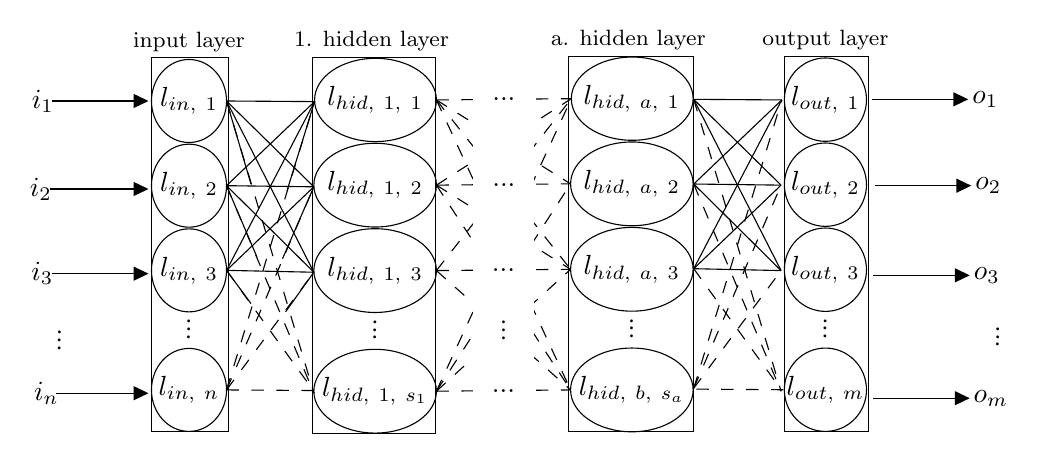
\begin{tikzpicture}[x=0.75pt,y=0.75pt,yscale=-0.8,xscale=0.8]
%uncomment if require: \path (0,300); %set diagram left start at 0, and has height of 300

%Shape: Rectangle [id:dp5348683704419017] 
\draw   (76.28,62) -- (122.66,62) -- (122.66,287) -- (76.28,287) -- cycle ;
%Shape: Ellipse [id:dp939731478529126] 
\draw   (76.28,88) .. controls (76.28,74.19) and (86.4,63) .. (98.88,63) .. controls (111.36,63) and (121.49,74.19) .. (121.49,88) .. controls (121.49,101.81) and (1 11.36,113) .. (98.88,113) .. controls (86.4,113) and (76.28,101.81) .. (76.28,88) -- cycle ;
%Shape: Ellipse [id:dp5664589230881223] 
\draw   (76.28,139) .. controls (76.28,125.19) and (86.4,114) .. (98.88,114) .. controls (111.36,114) and (121.49,125.19) .. (121.49,139) .. controls (121.49,152.81) and (111.36,164) .. (98.88,164) .. controls (86.4,164) and (76.28,152.81) .. (76.28,139) -- cycle ;

%Shape: Ellipse [id:dp7228345414575519] 
\draw   (76.28,190) .. controls (76.28,176.19) and (86.4,165) .. (98.88,165) .. controls (111.36,165) and (121.49,176.19) .. (121.49,190) .. controls (121.49,203.81) and (111.36,215) .. (98.88,215) .. controls (86.4,215) and (76.28,203.81) .. (76.28,190) -- cycle ;

%Shape: Ellipse [id:dp6381471751303389] 
\draw   (76.28,262) .. controls (76.28,248.19) and (86.4,237) .. (98.88,237) .. controls (111.36,237) and (121.49,248.19) .. (121.49,262) .. controls (121.49,275.81) and (111.36,287) .. (98.88,287) .. controls (86.4,287) and (76.28,275.81) .. (76.28,262) -- cycle ;

%Straight Lines [id:da0033305459292130024] 
\draw    (16.49,88) -- (71.47,88) ;
\draw [shift={(74.47,88)}, rotate = 180] [fill={rgb, 255:red, 0; green, 0; blue, 0 }  ][line width=0.08]  [draw opacity=0] (8.93,-4.29) -- (0,0) -- (8.93,4.29) -- cycle    ;

%Straight Lines [id:da5101048873615364] 
\draw    (15.34,141) -- (71.47,141) ;
\draw [shift={(74.47,141)}, rotate = 180] [fill={rgb, 255:red, 0; green, 0; blue, 0 }  ][line width=0.08]  [draw opacity=0] (8.93,-4.29) -- (0,0) -- (8.93,4.29) -- cycle    ;

%Straight Lines [id:da6465200926879782] 
\draw    (16.21,192) -- (71.47,192) ;
\draw [shift={(74.47,192)}, rotate = 180] [fill={rgb, 255:red, 0; green, 0; blue, 0 }  ][line width=0.08]  [draw opacity=0] (8.93,-4.29) -- (0,0) -- (8.93,4.29) -- cycle    ;

%Straight Lines [id:da5162655773532001] 
\draw    (19.05,264) -- (71.47,264) ;
\draw [shift={(74.47,264)}, rotate = 180] [fill={rgb, 255:red, 0; green, 0; blue, 0 }  ][line width=0.08]  [draw opacity=0] (8.93,-4.29) -- (0,0) -- (8.93,4.29) -- cycle    ;

%Shape: Rectangle [id:dp18972253282167162] 
\draw   (173.05,62) -- (247.44,62) -- (247.44,288) -- (173.05,288) -- cycle ;
%Shape: Ellipse [id:dp7229152371524696] 
\draw   (174.52,87.37) .. controls (174.52,73.53) and (190.94,62.3) .. (211.2,62.3) .. controls (231.46,62.3) and (247.88,73.53) .. (247.88,87.37) .. controls (247.88,101.22) and (231.46,112.45) .. (211.2,112.45) .. controls (190.94,112.45) and (174.52,101.22) .. (174.52,87.37) -- cycle ;
%Shape: Ellipse [id:dp5195092025670933] 
\draw   (174.08,138.68) .. controls (174.08,124.75) and (190.6,113.46) .. (210.98,113.46) .. controls (231.36,113.46) and (247.88,124.75) .. (247.88,138.68) .. controls (247.88,152.61) and (231.36,163.9) .. (210.98,163.9) .. controls (190.6,163.9) and (174.08,152.61) .. (174.08,138.68) -- cycle ;
%Shape: Ellipse [id:dp45163062887236016] 
\draw   (174.08,190.13) .. controls (174.08,176.2) and (190.6,164.91) .. (210.98,164.91) .. controls (231.36,164.91) and (247.88,176.2) .. (247.88,190.13) .. controls (247.88,204.06) and (231.36,215.36) .. (210.98,215.36) .. controls (190.6,215.36) and (174.08,204.06) .. (174.08,190.13) -- cycle ;
%Shape: Ellipse [id:dp6104698680122025] 
\draw   (174.08,262.78) .. controls (174.08,248.85) and (190.6,237.55) .. (210.98,237.55) .. controls (231.36,237.55) and (247.88,248.85) .. (247.88,262.78) .. controls (247.88,276.71) and (231.36,288) .. (210.98,288) .. controls (190.6,288) and (174.08,276.71) .. (174.08,262.78) -- cycle ;
%Shape: Rectangle [id:dp3256666346119699] 
\draw   (327.67,61.22) -- (402.96,61.22) -- (402.96,287.22) -- (327.67,287.22) -- cycle ;
%Shape: Ellipse [id:dp5309517723311545] 
\draw   (329.14,86.6) .. controls (329.14,72.75) and (345.56,61.53) .. (365.82,61.53) .. controls (386.07,61.53) and (402.49,72.75) .. (402.49,86.6) .. controls (402.49,100.44) and (386.07,111.67) .. (365.82,111.67) .. controls (345.56,111.67) and (329.14,100.44) .. (329.14,86.6) -- cycle ;
%Shape: Ellipse [id:dp4644453089406313] 
\draw   (328.7,137.9) .. controls (328.7,123.97) and (345.22,112.68) .. (365.6,112.68) .. controls (385.97,112.68) and (402.49,123.97) .. (402.49,137.9) .. controls (402.49,151.83) and (385.97,163.13) .. (365.6,163.13) .. controls (345.22,163.13) and (328.7,151.83) .. (328.7,137.9) -- cycle ;
%Shape: Ellipse [id:dp8559292750865175] 
\draw   (328.7,189.36) .. controls (328.7,175.43) and (345.22,164.13) .. (365.6,164.13) .. controls (385.97,164.13) and (402.49,175.43) .. (402.49,189.36) .. controls (402.49,203.29) and (385.97,214.58) .. (365.6,214.58) .. controls (345.22,214.58) and (328.7,203.29) .. (328.7,189.36) -- cycle ;
%Shape: Ellipse [id:dp1970629242881392] 
\draw   (328.7,262) .. controls (328.7,248.07) and (345.22,236.78) .. (365.6,236.78) .. controls (385.97,236.78) and (402.49,248.07) .. (402.49,262) .. controls (402.49,275.93) and (385.97,287.22) .. (365.6,287.22) .. controls (345.22,287.22) and (328.7,275.93) .. (328.7,262) -- cycle ;
%Shape: Rectangle [id:dp7142888753284027] 
\draw   (457.44,61.09) -- (508.19,61.09) -- (508.19,287) -- (457.44,287) -- cycle ;
%Shape: Ellipse [id:dp7295760206982997] 
\draw   (457.44,87.19) .. controls (457.44,73.33) and (468.51,62.09) .. (482.17,62.09) .. controls (495.83,62.09) and (506.9,73.33) .. (506.9,87.19) .. controls (506.9,101.05) and (495.83,112.29) .. (482.17,112.29) .. controls (468.51,112.29) and (457.44,101.05) .. (457.44,87.19) -- cycle ;
%Shape: Ellipse [id:dp4100384195259268] 
\draw   (457.44,138.4) .. controls (457.44,124.54) and (468.51,113.3) .. (482.17,113.3) .. controls (495.83,113.3) and (506.9,124.54) .. (506.9,138.4) .. controls (506.9,152.26) and (495.83,163.5) .. (482.17,163.5) .. controls (468.51,163.5) and (457.44,152.26) .. (457.44,138.4) -- cycle ;

%Shape: Ellipse [id:dp7445535886007981] 
\draw   (457.44,189.61) .. controls (457.44,175.74) and (468.51,164.5) .. (482.17,164.5) .. controls (495.83,164.5) and (506.9,175.74) .. (506.9,189.61) .. controls (506.9,203.47) and (495.83,214.71) .. (482.17,214.71) .. controls (468.51,214.71) and (457.44,203.47) .. (457.44,189.61) -- cycle ;

%Shape: Ellipse [id:dp5696755418086674] 
\draw   (457.44,261.9) .. controls (457.44,248.04) and (468.51,236.8) .. (482.17,236.8) .. controls (495.83,236.8) and (506.9,248.04) .. (506.9,261.9) .. controls (506.9,275.76) and (495.83,287) .. (482.17,287) .. controls (468.51,287) and (457.44,275.76) .. (457.44,261.9) -- cycle ;
%Straight Lines [id:da18885212790099604] 
\draw    (511.09,267) -- (566.07,267) ;
\draw [shift={(569.07,267)}, rotate = 180] [fill={rgb, 255:red, 0; green, 0; blue, 0 }  ][line width=0.08]  [draw opacity=0] (8.93,-4.29) -- (0,0) -- (8.93,4.29) -- cycle    ;

%Straight Lines [id:da35087841460038605] 
\draw    (510.19,87) -- (565.16,87) ;
\draw [shift={(568.16,87)}, rotate = 180] [fill={rgb, 255:red, 0; green, 0; blue, 0 }  ][line width=0.08]  [draw opacity=0] (8.93,-4.29) -- (0,0) -- (8.93,4.29) -- cycle    ;

%Straight Lines [id:da5340215529143741] 
\draw    (511.99,139) -- (566.97,139) ;
\draw [shift={(569.97,139)}, rotate = 180] [fill={rgb, 255:red, 0; green, 0; blue, 0 }  ][line width=0.08]  [draw opacity=0] (8.93,-4.29) -- (0,0) -- (8.93,4.29) -- cycle    ;

%Straight Lines [id:da6816101523134108] 
\draw    (511.09,193) -- (566.07,193) ;
\draw [shift={(569.07,193)}, rotate = 180] [fill={rgb, 255:red, 0; green, 0; blue, 0 }  ][line width=0.08]  [draw opacity=0] (8.93,-4.29) -- (0,0) -- (8.93,4.29) -- cycle    ;

%Straight Lines [id:da07173699686933155] 
\draw  [dash pattern={on 4.5pt off 4.5pt}]  (121.49,88) -- (174.08,263.78) ;
%Straight Lines [id:da6699097779078262] 
\draw  [dash pattern={on 4.5pt off 4.5pt}]  (121.49,262) -- (174.08,191.13) ;
%Straight Lines [id:da1642802446958136] 
\draw  [dash pattern={on 4.5pt off 4.5pt}]  (121.49,262) -- (174.08,139.68) ;
%Straight Lines [id:da1882795920867577] 
\draw  [dash pattern={on 4.5pt off 4.5pt}]  (121.49,262) -- (174.52,88.37) ;
%Straight Lines [id:da21393539615592538] 
\draw    (121.49,88) -- (174.52,88.37) ;
%Straight Lines [id:da4487867895893247] 
\draw    (121.49,88) -- (174.08,139.68) ;
%Straight Lines [id:da07147649974582793] 
\draw    (121.49,88) -- (174.08,191.13) ;
%Straight Lines [id:da29330792079044166] 
\draw    (121.49,139) -- (174.52,88.37) ;
%Straight Lines [id:da49448158210002213] 
\draw  [dash pattern={on 4.5pt off 4.5pt}]  (121.49,190) -- (174.08,262.78) ;
%Straight Lines [id:da09798373867862575] 
\draw    (121.49,139) -- (174.08,191.13) ;
%Straight Lines [id:da5600404631656062] 
\draw  [dash pattern={on 4.5pt off 4.5pt}]  (121.49,139) -- (174.08,263.78) ;
%Straight Lines [id:da7057392759609711] 
\draw    (121.49,190) -- (174.52,88.37) ;
%Straight Lines [id:da2885366017727522] 
\draw    (121.49,190) -- (174.08,139.68) ;
%Straight Lines [id:da34302481014830266] 
\draw    (121.49,190) -- (174.08,191.13) ;
%Straight Lines [id:da3967598060261417] 
\draw    (121.49,139) -- (174.08,139.68) ;
%Straight Lines [id:da2561105605921401] 
\draw    (121.49,88) -- (136.22,138) ;
%Straight Lines [id:da0846780391827735] 
\draw    (174.52,88.37) -- (157.92,142) ;
%Straight Lines [id:da8561394015640085] 
\draw    (174.08,139.68) -- (155.21,183) ;
%Straight Lines [id:da7742955999004255] 
\draw    (174.08,191.13) -- (157.02,215) ;
%Straight Lines [id:da3741138292647084] 
\draw    (121.49,139) -- (139.84,182) ;
%Straight Lines [id:da19823177683211468] 
\draw    (121.49,190) -- (136.22,210) ;
%Straight Lines [id:da7799354395016436] 
\draw  [dash pattern={on 4.5pt off 4.5pt}]  (247.88,87.37) -- (329.14,86.6) ;
%Straight Lines [id:da8112635885919046] 
\draw  [dash pattern={on 4.5pt off 4.5pt}]  (247.88,87.37) -- (328.7,137.9) ;
%Straight Lines [id:da43416826759224025] 
\draw  [dash pattern={on 4.5pt off 4.5pt}]  (247.88,87.37) -- (328.7,189.36) ;
%Straight Lines [id:da5962912105851825] 
\draw  [dash pattern={on 4.5pt off 4.5pt}]  (247.88,87.37) -- (328.7,262) ;
%Straight Lines [id:da414758159631222] 
\draw  [dash pattern={on 4.5pt off 4.5pt}]  (247.88,138.68) -- (328.7,137.9) ;
%Straight Lines [id:da4655355837425297] 
\draw  [dash pattern={on 4.5pt off 4.5pt}]  (247.88,138.68) -- (329.14,86.6) ;
%Straight Lines [id:da19554879472652642] 
\draw  [dash pattern={on 4.5pt off 4.5pt}]  (247.88,138.68) -- (328.7,189.36) ;
%Straight Lines [id:da5323232176676549] 
\draw  [dash pattern={on 4.5pt off 4.5pt}]  (247.88,138.68) -- (328.7,262) ;
%Straight Lines [id:da6152630037551357] 
\draw  [dash pattern={on 4.5pt off 4.5pt}]  (247.88,190.13) -- (329.14,86.6) ;
%Straight Lines [id:da7928666915958094] 
\draw  [dash pattern={on 4.5pt off 4.5pt}]  (247.88,190.13) -- (328.7,262) ;
%Straight Lines [id:da37586727330985115] 
\draw  [dash pattern={on 4.5pt off 4.5pt}]  (247.88,190.13) -- (328.7,189.36) ;
%Straight Lines [id:da7715167325292387] 
\draw  [dash pattern={on 4.5pt off 4.5pt}]  (247.88,262.78) -- (328.7,262) ;
%Straight Lines [id:da8147553751065622] 
\draw  [dash pattern={on 4.5pt off 4.5pt}]  (247.88,262.78) -- (328.7,189.36) ;
%Straight Lines [id:da8607258541912663] 
\draw  [dash pattern={on 4.5pt off 4.5pt}]  (247.88,262.78) -- (328.7,137.9) ;
%Straight Lines [id:da4710290973854665] 
\draw  [dash pattern={on 4.5pt off 4.5pt}]  (247.88,262.78) -- (329.14,86.6) ;
%Shape: Rectangle [id:dp8707492920309927] 
\draw  [draw opacity=0][fill={rgb, 255:red, 255; green, 255; blue, 255 }  ,fill opacity=1 ] (269.75,74.69) -- (306.82,74.69) -- (306.82,274.69) -- (269.75,274.69) -- cycle ;
%Straight Lines [id:da789374598203767] 
\draw  [dash pattern={on 4.5pt off 4.5pt}]  (402.86,87) -- (455.46,262.78) ;
%Straight Lines [id:da5608607968941501] 
\draw  [dash pattern={on 4.5pt off 4.5pt}]  (402.86,261) -- (455.46,190.13) ;
%Straight Lines [id:da8173621393477881] 
\draw  [dash pattern={on 4.5pt off 4.5pt}]  (402.86,261) -- (455.46,138.68) ;
%Straight Lines [id:da42024579143459984] 
\draw  [dash pattern={on 4.5pt off 4.5pt}]  (402.86,261) -- (455.9,87.37) ;
%Straight Lines [id:da4970992533092691] 
\draw    (402.86,87) -- (455.9,87.37) ;
%Straight Lines [id:da5336499941942965] 
\draw    (402.86,87) -- (455.46,138.68) ;
%Straight Lines [id:da6837746318616225] 
\draw    (402.86,87) -- (455.46,190.13) ;
%Straight Lines [id:da2450666544795037] 
\draw    (402.86,138) -- (455.9,87.37) ;
%Straight Lines [id:da54432464900309] 
\draw  [dash pattern={on 4.5pt off 4.5pt}]  (402.86,189) -- (455.46,261.78) ;
%Straight Lines [id:da9110502437081351] 
\draw    (402.86,138) -- (455.46,190.13) ;
%Straight Lines [id:da18057385661891412] 
\draw  [dash pattern={on 4.5pt off 4.5pt}]  (402.86,138) -- (455.46,262.78) ;
%Straight Lines [id:da613380831677923] 
\draw    (402.86,189) -- (455.9,87.37) ;
%Straight Lines [id:da6296455944188728] 
\draw    (402.86,189) -- (455.46,138.68) ;
%Straight Lines [id:da11572374477508784] 
\draw    (402.86,189) -- (455.46,190.13) ;
%Straight Lines [id:da17311782425039035] 
\draw    (402.86,138) -- (455.46,138.68) ;

%Straight Lines [id:da6430113077352528] 
\draw  [dash pattern={on 4.5pt off 4.5pt}]  (121.49,262) -- (174.52,262.37) ;
%Straight Lines [id:da7394517258615123] 
\draw  [dash pattern={on 4.5pt off 4.5pt}]  (404.4,261.52) -- (457.44,261.9) ;

% Text Node
\draw (570.06,193) node [anchor=west] [inner sep=0.75pt]   [align=left] {$\displaystyle o_{3}$};
% Text Node
\draw (570.96,139) node [anchor=west] [inner sep=0.75pt]   [align=left] {$\displaystyle o_{2}$};
% Text Node
\draw (569.16,87) node [anchor=west] [inner sep=0.75pt]   [align=left] {$\displaystyle o_{1}$};
% Text Node
\draw (569.87,267) node [anchor=west] [inner sep=0.75pt]   [align=left] {$\displaystyle o_{m}$};
% Text Node
\draw (482.17,189.61) node   [align=left] {$\displaystyle l_{out,\ 3}$};
% Text Node
\draw (482.17,138.4) node   [align=left] {$\displaystyle l_{out,\ 2}$};
% Text Node
\draw (22.03,264) node [anchor=east] [inner sep=0.75pt]   [align=left] {$\displaystyle i_{n}$};
% Text Node
\draw (18.72,192) node [anchor=east] [inner sep=0.75pt]   [align=left] {$\displaystyle i_{3}$};
% Text Node
\draw (17.78,141) node [anchor=east] [inner sep=0.75pt]   [align=left] {$\displaystyle i_{2}$};
% Text Node
\draw (19.02,88) node [anchor=east] [inner sep=0.75pt]   [align=left] {$\displaystyle i_{1}$};
% Text Node
\draw (98.88,262) node   [align=left] {$\displaystyle l_{in,\ n}$};
% Text Node
\draw (98.88,190) node   [align=left] {$\displaystyle l_{in,\ 3}$};
% Text Node
\draw (98.88,139) node   [align=left] {$\displaystyle l_{in,\ 2}$};
% Text Node
\draw (98.88,88) node   [align=left] {$\displaystyle l_{in,\ 1}$};
% Text Node
\draw (482.14,216.71) node [anchor=west] [inner sep=0.75pt]  [rotate=-91.1] [align=left] {...};
% Text Node
\draw (482.17,59.04) node [anchor=south] [inner sep=0.75pt]  [font=\footnotesize] [align=left] {output layer};
% Text Node
\draw (482.17,261.9) node   [align=left] {$\displaystyle l_{out,\ m}$};
% Text Node
\draw (482.17,87.19) node   [align=left] {$\displaystyle l_{out,\ 1}$};
% Text Node
\draw (365.6,86.45) node   [align=left] {$\displaystyle l_{hid,\ a,\ 1}$};
% Text Node
\draw (365.6,137.9) node   [align=left] {$\displaystyle l_{hid,\ a,\ 2}$};
% Text Node
\draw (365.6,189.36) node   [align=left] {$\displaystyle l_{hid,\ a,\ 3}$};
% Text Node
\draw (365.6,262) node   [align=left] {$\displaystyle l_{hid,\ b,\ s_{a}}$};
% Text Node
\draw (365.43,216.58) node [anchor=west] [inner sep=0.75pt]  [rotate=-90] [align=left] {...};
% Text Node
\draw (365.82,58.53) node [anchor=south] [inner sep=0.75pt]  [font=\footnotesize] [align=left] {a. hidden layer };
% Text Node
\draw (210.95,217.36) node [anchor=west] [inner sep=0.75pt]  [rotate=-91.1] [align=left] {...};
% Text Node
\draw (210.98,262.78) node   [align=left] {$\displaystyle l_{hid,\ 1,\ s_{1}}$};
% Text Node
\draw (210.98,190.13) node   [align=left] {$\displaystyle l_{hid,\ 1,\ 3}$};
% Text Node
\draw (210.98,138.68) node   [align=left] {$\displaystyle l_{hid,\ 1,\ 2}$};
% Text Node
\draw (210.98,87.22) node   [align=left] {$\displaystyle l_{hid,\ 1,\ 1}$};
% Text Node
\draw (211.2,59.3) node [anchor=south] [inner sep=0.75pt]  [font=\footnotesize] [align=left] {1. hidden layer };
% Text Node
\draw (588.55,221.66) node [anchor=north west][inner sep=0.75pt]  [rotate=-91.1] [align=left] {...};
% Text Node
\draw (23.42,223.66) node [anchor=north west][inner sep=0.75pt]  [rotate=-91.1] [align=left] {...};
% Text Node
\draw (98.85,217) node [anchor=west] [inner sep=0.75pt]  [rotate=-91.1] [align=left] {...};
% Text Node
\draw (98.88,60) node [anchor=south] [inner sep=0.75pt]  [font=\footnotesize] [align=left] {input layer};
% Text Node
\draw (288.51,86.99) node   [align=left] {...};
% Text Node
\draw (288.51,138.37) node   [align=left] {...};
% Text Node
\draw (288.29,189.75) node   [align=left] {...};
% Text Node
\draw (288.29,262.39) node   [align=left] {...};
% Text Node
\draw (288.29,226.07) node  [rotate=-90.15] [align=left] {...};


\end{tikzpicture}


\end{center}
\caption{The relation between the different layers.}
\label{neuronal_layer_relation}
\end{figure}

The \gls{neuronal network} consists of all parts mentioned before, as can be seen in Figure \ref{neuronal_layer_relation}. Every circle or ellipse represents one neuron. The first  \gls{layer} is the \gls{input layer} and has as many nodes, as the \gls{input size} $n$. This means if you want to forward binary information of four variables, the  \gls{input} size and therefore the \gls{input layer} would be in the size of four \glspl{neuron}. This also holds for the \gls{output layer size}, which is denoted by $m$. 
The \gls{amount of hidden layers} $a$ and its size $s$ can be chosen arbitrarily. Although there are no constraints for the \glspl{hidden layer}, the amount and size can hugely affect the efficiency and capability to learn.
\begin{figure}[ht]
\begin{center}
\label{neuron}
\tikzset{every picture/.style={line width=0.75pt}} %set default line width to 0.75pt    
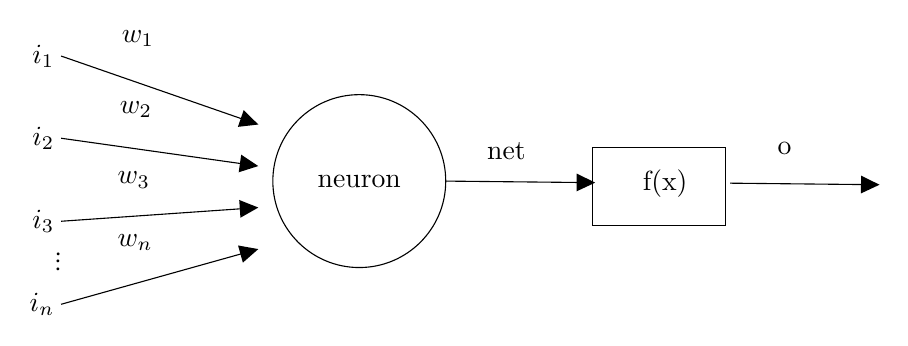
\begin{tikzpicture}[x=0.75pt,y=0.75pt,yscale=-1,xscale=1]
%uncomment if require: \path (0,300); %set diagram left start at 0, and has height of 300

%Shape: Circle [id:dp8788298950890718] 
\draw   (226,121.65) .. controls (226,98.65) and (244.65,80) .. (267.65,80) .. controls (290.65,80) and (309.3,98.65) .. (309.3,121.65) .. controls (309.3,144.65) and (290.65,163.3) .. (267.65,163.3) .. controls (244.65,163.3) and (226,144.65) .. (226,121.65) -- cycle ;
%Straight Lines [id:da3838769529758834] 
\draw    (124,101) -- (216.03,113.98) ;
\draw [shift={(219,114.4)}, rotate = 188.03] [fill={rgb, 255:red, 0; green, 0; blue, 0 }  ][line width=0.08]  [draw opacity=0] (8.93,-4.29) -- (0,0) -- (8.93,4.29) -- cycle    ;
%Straight Lines [id:da23619311043896896] 
\draw    (124,141) -- (216.01,134.61) ;
\draw [shift={(219,134.4)}, rotate = 536.03] [fill={rgb, 255:red, 0; green, 0; blue, 0 }  ][line width=0.08]  [draw opacity=0] (8.93,-4.29) -- (0,0) -- (8.93,4.29) -- cycle    ;
%Straight Lines [id:da4533097231798262] 
\draw    (124,181) -- (216.11,155.21) ;
\draw [shift={(219,154.4)}, rotate = 524.36] [fill={rgb, 255:red, 0; green, 0; blue, 0 }  ][line width=0.08]  [draw opacity=0] (8.93,-4.29) -- (0,0) -- (8.93,4.29) -- cycle    ;
%Straight Lines [id:da017364411003136793] 
\draw    (124,61.4) -- (216.17,93.42) ;
\draw [shift={(219,94.4)}, rotate = 199.16] [fill={rgb, 255:red, 0; green, 0; blue, 0 }  ][line width=0.08]  [draw opacity=0] (8.93,-4.29) -- (0,0) -- (8.93,4.29) -- cycle    ;
%Straight Lines [id:da2738426817104591] 
\draw    (309.3,121.65) -- (378.3,122.37) ;
\draw [shift={(381.3,122.4)}, rotate = 180.6] [fill={rgb, 255:red, 0; green, 0; blue, 0 }  ][line width=0.08]  [draw opacity=0] (8.93,-4.29) -- (0,0) -- (8.93,4.29) -- cycle    ;
%Shape: Rectangle [id:dp15584865208252952] 
\draw   (380,105.4) -- (444.3,105.4) -- (444.3,143) -- (380,143) -- cycle ;
%Straight Lines [id:da6312953564844079] 
\draw    (446.3,122.65) -- (515.3,123.37) ;
\draw [shift={(518.3,123.4)}, rotate = 180.6] [fill={rgb, 255:red, 0; green, 0; blue, 0 }  ][line width=0.08]  [draw opacity=0] (8.93,-4.29) -- (0,0) -- (8.93,4.29) -- cycle    ;

% Text Node
\draw (267.65,121.65) node   [align=left] {neuron};
% Text Node
\draw (122,61.4) node [anchor=east] [inner sep=0.75pt]   [align=left] {$\displaystyle i_{1}$};
% Text Node
\draw (122,141) node [anchor=east] [inner sep=0.75pt]   [align=left] {$\displaystyle i_{3}$};
% Text Node
\draw (122,101) node [anchor=east] [inner sep=0.75pt]   [align=left] {$\displaystyle i_{2}$};
% Text Node
\draw (122,181) node [anchor=east] [inner sep=0.75pt]   [align=left] {$\displaystyle i_{n}$};
% Text Node
\draw (124.63,153.66) node [anchor=north west][inner sep=0.75pt]  [rotate=-91.1] [align=left] {...};
% Text Node
\draw (152,48) node [anchor=north west][inner sep=0.75pt]   [align=left] {$\displaystyle w_{1}$};
% Text Node
\draw (151,82) node [anchor=north west][inner sep=0.75pt]   [align=left] {$\displaystyle w_{2}$};
% Text Node
\draw (150,146) node [anchor=north west][inner sep=0.75pt]   [align=left] {$\displaystyle w_{n}$};
% Text Node
\draw (150,116) node [anchor=north west][inner sep=0.75pt]   [align=left] {$\displaystyle w_{3}$};
% Text Node
\draw (415,123) node   [align=left] {f(x)};
% Text Node
\draw (468,102) node [anchor=north west][inner sep=0.75pt]   [align=left] {o};
% Text Node
\draw (328,102) node [anchor=north west][inner sep=0.75pt]   [align=left] {net};
\end{tikzpicture}
\caption{A visualization of a neuron.}
\label{neuron_vis}
\end{center}
\end{figure}
In Figure \ref{neuron_vis}, the structure of a \gls{neuron} can be seen. The abbreviation $i$ stands for  \gls{input}, $w$ refers to \gls{weight} and $o$ to the \gls{output} of the neuron. The  \glspl{input} and \glspl{weight} can be described in the form of a \gls{vector}. The output $o$ gets weighted accordingly and functions as  \gls{input} for the following \glspl{neuron}. Each component represents one  \gls{input} or \gls{weight}. This yields the \glspl{vector} $\vec{i}$ and $\vec{w}$.
\begin{align}
\vec{i} = \begin{pmatrix} 
i_{1}\\ 
i_{2}\\ 
\ldots \\ 
i_{n}
\end{pmatrix}
&&
\vec{w} = \begin{pmatrix}
w_{1}\\ 
w_{2}\\ 
\ldots \\ 
w_{n}
\end{pmatrix}
\label{def_vector}
\end{align}
The sum, in figure \ref{neuron_vis} referenced as net, is determined by the weighted summation of all the  \glspl{input}. 
\begin{equation}
  \sum_{x = 1}^{n} i_{x} \cdot w_{x}  
  \label{net_sum}
\end{equation}
The equation \ref{net_sum} shows the \gls{net value} in the form of a sum.
Due to the properties of the \gls{scalar product}, this sum can be rewritten in the form of this \gls{vector} operation:
\begin{equation}
net = \vec{i}  \vec{w}
\label{net_scal}
\end{equation}
This weighted sum gets forwarded to the \gls{activation function}. By replacing the \gls{net value} with the definition stated in equation \ref{net_scal}  and $f(x)$ being the \gls{activation function}, the output is defined as follows:
\begin{equation}
\begin{gathered}
       o = f(net)\\
    o = f(\vec{i} \cdot \vec{w}) 
\end{gathered}
\end{equation}
The final output, or an intermediate result, of a \gls{hidden layer} can also be described in a vector form.
\begin{equation}
\begin{gathered}
      \begin{pmatrix}
o_{1}\\ 
o_{2}\\ 
...\\ 
o_{m}
\end{pmatrix} = \begin{pmatrix}
f(net_{1})\\ 
f(net_{2})\\ 
...\\ 
f(net_{m})
\end{pmatrix}
\end{gathered}
\end{equation}
As one can see in formula \ref{net_scal}, the \gls{net value} can also be described in a vector form. By expanding the stated definition, it can be formulated such that multiple values are defined in one \gls{vector}. Although it yields the same result, the output \gls{vector} $\vec{o}$ can be calculated easier, when using \glspl{net value} in a vector form.
\begin{equation}
    \begin{pmatrix}net_{1}\\ net_{2}\\ ...\\ net_{m}\end{pmatrix} =\begin{pmatrix}
w_{1, 1} & w_{2, 1}  & ... &w_{n,1} \\ 
w_{1, 2} & w_{2, 2} & ... & w_{n,2} \\ 
... & ... &  ... & ...\\ 
w_{1,s} & w_{2, s} & ...  & w_{n, s}
\end{pmatrix} \cdot \begin{pmatrix}
i_{1}\\ 
i_{2}\\ 
...\\
i_{n}
\end{pmatrix}
\label{out_vector}
\end{equation}
Formula \ref{out_vector} is a stacked up version of equation \ref{net_scal}. Every row represents all the \glspl{weight} from one specific neuron. The output of this \gls{neuron} is used as  \gls{input} in the next one. It acts as output as well as an  \gls{input}, but nevertheless, it is denoted by $i$. A noticeable remark is, that it fits with the definition of the \gls{scalar product}, which requires the dimension of the first \gls{vector} to be the same as the dimension of the second \gls{vector}. Which is the case, as it can be seen. The letter $s$ denotes the \gls{size} of the layer, from which the output gets calculated of.
However, there are different kinds of \glspl{neuron}, depending on their \glspl{activation function}. Depending on the context, different functions are more efficient to use. The most common and popular types of such are:  \cite{neuronal_network}
\begin{figure}[H]%
\label{activation_function}
\begin{minipage}[t]{0.5\textwidth}
\begin{center}
\textbf{Linear}
\begin{equation}\nonumber
    f(x) = x
\end{equation}\newline
\begin{tikzpicture}[scale = 0.5]
\begin{axis}[
  axis x line=center,
  axis y line=center,
  xlabel={$x$},
  ylabel={$y$},
  xlabel style={below right},
  ylabel style={above left},
  xmin=-3,
  xmax=3,
  ymin=-3,
  ymax=3]
\addplot [mark=none,domain=-2.5:2.5] {x};
\end{axis}
\end{tikzpicture}\\
Mostly used in \gls{input layer}.
\end{center}
\end{minipage}
\begin{minipage}[t]{0.5\textwidth}
\begin{center}
\textbf{Sigmoid}
\begin{equation}\nonumber
    f(x) = \frac{1}{1 + e^{-x}}
\end{equation}
\begin{tikzpicture}[scale = 0.5]
\begin{axis}[
  axis x line=center,
  axis y line=center,
  xlabel={$x$},
  ylabel={$y$},
  xlabel style={below right},
  ylabel style={above left},
  xmin=-3.5,
  xmax=3.5,
  ymin=-3.5,
  ymax=3.5]
\addplot [mark=none,domain=-3:3] {1/(1+(e^-x))};
\end{axis}
\end{tikzpicture}\\
Mostly used in \glspl{hidden layer}.
\end{center}
\end{minipage}

\vspace{1cm}
\begin{minipage}[t]{0.5\textwidth}
\begin{center}
\textbf{Rectified linear unit (ReLU)}
\begin{equation}\nonumber
f(x) \left\{\begin{matrix}
0 \text{ for } x \leq 0\\ 
x \text{ for } x >  0
\end{matrix}\right.
\end{equation}
\begin{tikzpicture}[scale = 0.5]
\begin{axis}[
  axis x line=center,
  axis y line=center,
  xlabel={$x$},
  ylabel={$y$},
  xlabel style={below right},
  ylabel style={above left},
  xmin=-3,
  xmax=3,
  ymin=-3,
  ymax=3]
\addplot [mark=none,domain=-2.5:0] {0};
\addplot [mark=none,domain=0:2.5] {x};
\end{axis}
\end{tikzpicture}\\
Mostly used in \glspl{hidden layer}.
\end{center}
\end{minipage}
\begin{minipage}[t]{0.5\textwidth}
\begin{center}
\textbf{Binary step}
\begin{equation}\nonumber
f(x) \left\{\begin{matrix}
0 \text{ for } x < 0\\ 
1 \text{ for } x \geq 0
\end{matrix}\right.
\end{equation}
\begin{tikzpicture}[scale = 0.5]
\begin{axis}[
  axis x line=center,
  axis y line=center,
  xlabel={$x$},
  ylabel={$y$},
  xlabel style={below right},
  ylabel style={above left},
  xmin=-3,
  xmax=3,
  ymin=-3,
  ymax=3]
\addplot [mark=none,domain=-2.5:0] {0};
\addplot [mark=none,domain=0:2.5] {1};
\end{axis}
\end{tikzpicture}\\
Mostly used in  \glspl{output layer}.
\end{center}
\end{minipage}
\end{figure}
The derivative of these functions is important to make a learning process possible. It is used for the \gls{back propagation}. Therefore \gls{linear function} and \gls{binary step function} are not really used in the \glspl{hidden layer}.
Although the \gls{sigmoid neuron} is biologically more plausible, the \gls{ReLU} functions have shown to be more efficient for \glspl{hidden layer}. \cite{advantages_activation} \\
Sigmoid yields the property of always being finite whereas, \gls{ReLU} diverges into infinity. Additionally, the easily calculable derivative of \gls{ReLU} tends to converge faster to the wanted value. 
\subsubsection{Learning}\label{learning}
To learn, the \gls{neuronal network} gets optimized by changing the \glspl{weight} $w$. To change these values appropriately for the task given, a goal has to be set. This goal is important to calculate how much the actual output differs from the wanted results. It is denoted by $t$, which stands for \gls{target}. The \gls{neuronal network} can be compared to a function, which converts $n$ \glspl{input} to $m$ \glspl{output}.
\begin{equation}
    f(x_{1},x_{2},x_{3},...,x_{n}) \rightarrow (y_{1},y_{2},y_{3},...,y_{m})
\end{equation}
With the data given, the network compares the yielded \gls{output} values to the target values by calculating the error. A similar formula is used to calculate the variance in statistics.
\begin{equation}
   E = \frac{1}{m}\sum_{i=1}^{m}\left ( y_{i}- t_{i} \right )^{2}
\end{equation}
To make \gls{back propagation} possible, two of the three values (\gls{input}, \gls{output} and \gls{target}) have to be constant. When the \gls{input} \gls{vector} $\vec{i}$ and the target $\vec{t}$ are fixed, the only variable is $\vec{w}$. This can be used to analyze how much the \gls{output} differs from the \gls{target} for given \glspl{weight}. \\
Reformulating yields a function, which is only dependant on $\vec{w}$. By plugging this formula into the equation, which assigns the numerical error, it can be optimized to minimize the error. The function is denoted by:
\begin{equation}
E_{\;\vec{i}\;\vec{t}}(\vec{w})
\end{equation}
The \gls{optimization} happens due to the adjustment of the \glspl{weight}. As a result of the dependency, the \glspl{output} change with them. Which means by changing $\vec{w}$, we can achieve a \gls{convergence} or \gls{divergence} of the target values. So how does this happen?




\begin{centering}
\begin{figure}[ht]

\tikzset{every picture/.style={line width=0.75pt}} %set default line width to 0.75pt        

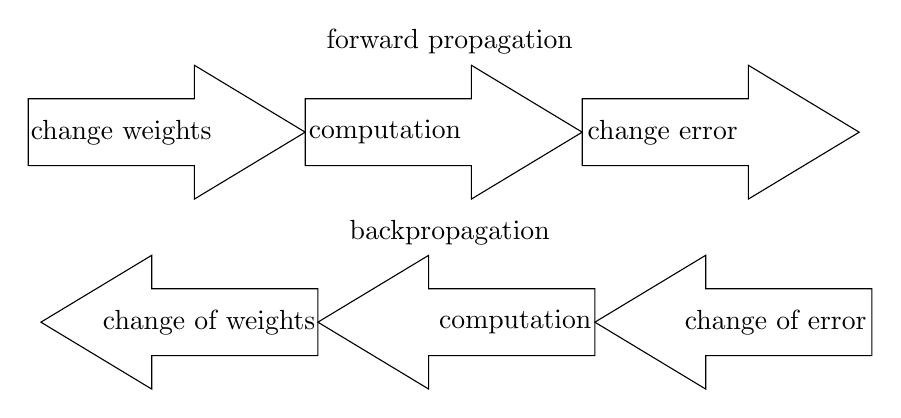
\begin{tikzpicture}[x=0.75pt,y=0.75pt,yscale=-1,xscale=1]
%uncomment if require: \path (0,300); %set diagram left start at 0, and has height of 300

%Right Arrow [id:dp22261738170682643] 
\draw   (82.95,58.11) -- (163.02,58.11) -- (163.02,42) -- (216.4,74.23) -- (163.02,106.45) -- (163.02,90.34) -- (82.95,90.34) -- cycle ;
%Right Arrow [id:dp3421608895508881] 
\draw   (216.4,58.11) -- (296.47,58.11) -- (296.47,42) -- (349.85,74.23) -- (296.47,106.45) -- (296.47,90.34) -- (216.4,90.34) -- cycle ;
%Right Arrow [id:dp4856504291402164] 
\draw   (349.85,58.11) -- (429.92,58.11) -- (429.92,42) -- (483.3,74.23) -- (429.92,106.45) -- (429.92,90.34) -- (349.85,90.34) -- cycle ;


%Right Arrow [id:dp6743816527001738] 
\draw   (489.41,181.89) -- (409.34,181.89) -- (409.34,198) -- (355.95,165.77) -- (409.34,133.55) -- (409.34,149.66) -- (489.41,149.66) -- cycle ;
%Right Arrow [id:dp6788485553692352] 
\draw   (355.95,181.89) -- (275.88,181.89) -- (275.88,198) -- (222.5,165.77) -- (275.88,133.55) -- (275.88,149.66) -- (355.95,149.66) -- cycle ;
%Right Arrow [id:dp8745803677179349] 
\draw   (222.5,181.89) -- (142.43,181.89) -- (142.43,198) -- (89.05,165.77) -- (142.43,133.55) -- (142.43,149.66) -- (222.5,149.66) -- cycle ;



% Text Node
\draw (488.08,165.77) node [anchor=east] [inner sep=0.75pt]   [align=left] {change of error};
% Text Node
\draw (355.51,165.77) node [anchor=east] [inner sep=0.75pt]   [align=left] {computation};
% Text Node
\draw (222.52,165.77) node [anchor=east] [inner sep=0.75pt]   [align=left] {change of weights};
% Text Node
\draw (82.94,74.23) node [anchor=west] [inner sep=0.75pt]   [align=left] {change weights};
% Text Node
\draw (216.85,74.23) node [anchor=west] [inner sep=0.75pt]   [align=left] {computation};
% Text Node
\draw (351.18,74.23) node [anchor=west] [inner sep=0.75pt]   [align=left] {change error};
% Text Node
\draw (286,38) node [anchor=south] [inner sep=0.75pt]   [align=left] {forward propagation};
% Text Node
\draw (286,130) node [anchor=south] [inner sep=0.75pt]   [align=left] {backpropagation};


\end{tikzpicture}
\caption{The difference between forward and back propagation.}
\label{backpropagation}
\end{figure}
\end{centering}

The forward propagation determines the change of the error when changing the weights. But when the weights should be optimized, backpropagation is used. As can be seen in Figure \ref{backpropagation}, the data gets passed in the opposite direction. So now, one can use the change of the error to get them according to the change of weights. This adjustment has to be made to yield a specific error. \\
The network should be doing better after this process, so the error should get smaller. In general, it does not matter how fast this value gets smaller. The function $E$ is multidimensional, which allocates the error to the input and weights. To be optimized, the \gls{gradient} can be used. This function is denoted by $\triangledown f$.  The \gls{gradient} of a more-dimensional function describes its steepest ascent. \cite{grad} \\\\
In this context the \gls{gradient} always points in the direction, where the error increases the most. This would lead to a \gls{divergence} of the \glspl{output} and the \glspl{target}. So the negative \gls{gradient} can be used to find the direction, in which the error decreases the fastest. Adding a multiple of the negative \gls{gradient} and the old \glspl{weight} together, the resulting \glspl{weight} are ensured to be closer to the target value than the old one. But this only holds when the factor, with which the \gls{gradient} gets multiplied with, is not too large. In the worst-case scenario, the new $\vec{w}$ does not perform better, because it overshoots the optimal point. Another unlucky case would be if the greatest descent of the function would lead to a local \gls{minimum}, which would achieve worse results than other minima. This can be prevented by fully optimizing the function multiple times with random \glspl{weight}. \\
To complete the learning process, the optimization has to be executed repeatedly until the \glspl{output} approximates the \glspl{target} sufficiently. Mathematically this step can be defined as follows:

\begin{equation} \label{opt_func}
    w_{new} = w_{old} - \alpha \cdot \triangledown f E(w_{old})
\end{equation}
The constant $\alpha$ is called \gls{learning rate} and defines how fast this approximation should happen. By choosing a large value, the trade-off for the time gained is the diminishing accuracy. The target values can be calculated in different ways which have their advantages and disadvantages. \\
For example, an \gls{AI}, which looks for patterns in pictures and has to state if the picture shows something specific. The \gls{target} then is defined by the data to be recognized, in our case an object. Therefore you would label all pictures according to which object is seen in the picture. The \gls{neuronal network} improves the ability to recognize this specific object or pattern with every picture shown, by comparing the actual label to the \gls{output} of the \gls{neuronal network}. An example would be, that it should recognize a dog in a picture. The network gets all the pixels of the pictures and the labels as \glspl{input}. It should \gls{output} 'dog' or 'not a dog'. By converting this label to a 0 for 'not a dog' and 1 for a 'dog', the numerical value can be used as the target value. By repeatedly showing pictures and recreating the optimization process stated in equation \ref{opt_func}, the network recognizes a dog increasingly better.
\subsubsection{Example}
Let's create an \gls{AI}, which can solve a simple task.\cite{NN_example} By doing so, the behaviour of a simple \gls{neuronal network} can be demonstrated. The task looks like the following. The input comes in the form of a list with three elements. Every element is determined by the number $0$ or $1$. The output the \gls{AI} should return, is one of the three numbers. Which number is determined by $a$. If, for example,  $a = 1$, then only the first number in the list is significant. So the output should be the same number as in the first element of the list. A few examples will be given below to demonstrate the output for each input.\\
\begin{minipage}{0.3\textwidth}
  \begin{align*}
    a = 1\\
\left [ 1,1,0 \right ] \rightarrowtail 1\\
\left [ 0,1,1 \right ] \rightarrowtail 0\\
\left [ 1,0,1 \right ] \rightarrowtail 1\\
\left [ 0,1,0 \right ] \rightarrowtail 0\\
  \end{align*} 
\end{minipage}
\begin{minipage}{0.3\textwidth}
  \begin{align*}
     a = 2\\
\left [ 1,1,0 \right ] \rightarrowtail 1\\
\left [ 0,1,1 \right ] \rightarrowtail 1\\
\left [ 1,0,1 \right ] \rightarrowtail 0\\
\left [ 0,1,0 \right ] \rightarrowtail 1\\
  \end{align*}
\end{minipage}
\begin{minipage}{0.3\textwidth}
  \begin{align*}
     a = 3\\
\left [ 1,1,0 \right ] \rightarrowtail 0\\
\left [ 0,1,1 \right ] \rightarrowtail 1\\
\left [ 1,0,1 \right ] \rightarrowtail 1\\
\left [ 0,1,0 \right ] \rightarrowtail 0\\
  \end{align*}
\end{minipage}\\
The network will receive the value exactly in the form shown above. So, for instance the list $ \left[ 1,1,0 \right ] $ and its goal $\rightarrowtail 1 $.  It is not clear, if this task can be solved with just one neuron. But to keep it simple, the first attempt will just have one \gls{neuron} in the \gls{hidden layer}. The \gls{input layer} will have the same size as the input itself. Which is three, hence three input numbers. The activation function is linear. This means the input won't be transformed. For this reason, we can assume there is no \gls{activation function} for this layer. The same counts for the \gls{output layer}. The goal is, to get one number returned, so the size will be one. \\
The network has in total four connections and five nodes. The three connections between the \gls{input layer} and \gls{hidden layer} have one weight each. In comparison the human brain has $10^{15}$ connections, which are called synapses. The amount of neurons in a human brain has been estimated to something around $10^{11}$. So the \gls{neuronal network} is primitive. Due to its simplicity the whole network can be sketched as it is shown below in fig \ref{networkexample}. 
\\
\begin{figure}[h]%
\tikzset{every picture/.style={line width=0.75pt}} %set default line width to 0.75pt        

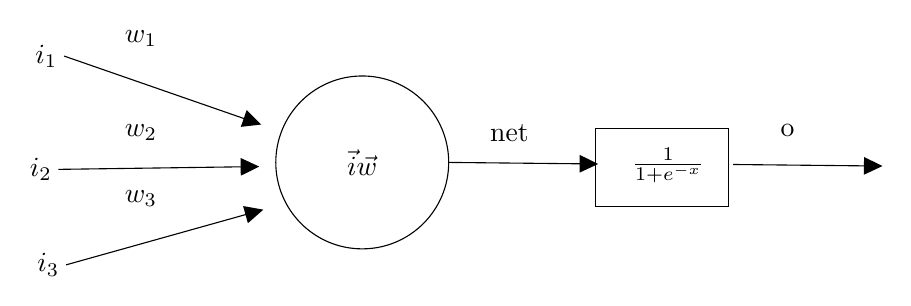
\begin{tikzpicture}[x=0.75pt,y=0.75pt,yscale=-1,xscale=1]
%uncomment if require: \path (0,300); %set diagram left start at 0, and has height of 300

%Shape: Circle [id:dp9348080173273374] 
\draw   (246,141.65) .. controls (246,118.65) and (264.65,100) .. (287.65,100) .. controls (310.65,100) and (329.3,118.65) .. (329.3,141.65) .. controls (329.3,164.65) and (310.65,183.3) .. (287.65,183.3) .. controls (264.65,183.3) and (246,164.65) .. (246,141.65) -- cycle ;
%Straight Lines [id:da1269091886653675] 
\draw    (145,191) -- (237.11,165.21) ;
\draw [shift={(240,164.4)}, rotate = 524.36] [fill={rgb, 255:red, 0; green, 0; blue, 0 }  ][line width=0.08]  [draw opacity=0] (8.93,-4.29) -- (0,0) -- (8.93,4.29) -- cycle    ;
%Straight Lines [id:da15349329279145918] 
\draw    (144,90.4) -- (236.17,122.42) ;
\draw [shift={(239,123.4)}, rotate = 199.16] [fill={rgb, 255:red, 0; green, 0; blue, 0 }  ][line width=0.08]  [draw opacity=0] (8.93,-4.29) -- (0,0) -- (8.93,4.29) -- cycle    ;

%Straight Lines [id:da5988826401793466] 
\draw    (329.3,141.65) -- (398.3,142.37) ;
\draw [shift={(401.3,142.4)}, rotate = 180.6] [fill={rgb, 255:red, 0; green, 0; blue, 0 }  ][line width=0.08]  [draw opacity=0] (8.93,-4.29) -- (0,0) -- (8.93,4.29) -- cycle    ;
%Shape: Rectangle [id:dp5962398579126695] 
\draw   (400,125.4) -- (464.3,125.4) -- (464.3,163) -- (400,163) -- cycle ;
%Straight Lines [id:da9702957838712694] 
\draw    (466.3,142.65) -- (535.3,143.37) ;
\draw [shift={(538.3,143.4)}, rotate = 180.6] [fill={rgb, 255:red, 0; green, 0; blue, 0 }  ][line width=0.08]  [draw opacity=0] (8.93,-4.29) -- (0,0) -- (8.93,4.29) -- cycle    ;
%Straight Lines [id:da8900223187436345] 
\draw    (141.3,145) -- (235,143.69) ;
\draw [shift={(238,143.65)}, rotate = 539.2] [fill={rgb, 255:red, 0; green, 0; blue, 0 }  ][line width=0.08]  [draw opacity=0] (8.93,-4.29) -- (0,0) -- (8.93,4.29) -- cycle    ;

% Text Node
\draw (287.65,141.65) node   [align=left] {$\vec{i}\vec{w} $};
% Text Node
\draw (139.3,145) node [anchor=east] [inner sep=0.75pt]   [align=left] {$\displaystyle i_{2}$};
% Text Node
\draw (172,122) node [anchor=north west][inner sep=0.75pt]   [align=left] {$\displaystyle w_{2}$};
% Text Node
\draw (435,143) node   [align=left] {$\frac{1}{1+e^{-x}}$};
% Text Node
\draw (488,122) node [anchor=north west][inner sep=0.75pt]   [align=left] {o};
% Text Node
\draw (348,122) node [anchor=north west][inner sep=0.75pt]   [align=left] {net};
% Text Node
\draw (142,90.4) node [anchor=east] [inner sep=0.75pt]   [align=left] {$\displaystyle i_{1}$};
% Text Node
\draw (172,77) node [anchor=north west][inner sep=0.75pt]   [align=left] {$\displaystyle w_{1}$};
% Text Node
\draw (143,191) node [anchor=east] [inner sep=0.75pt]   [align=left] {$\displaystyle i_{3}$};
% Text Node
\draw (172,154) node [anchor=north west][inner sep=0.75pt]   [align=left] {$\displaystyle w_{3}$};
\end{tikzpicture}
\caption{The structure of the neuronal network. It contains three \gls{input layer} nodes, one \gls{hidden layer} node and one \gls{output layer} node.}
\label{networkexample}
\end{figure}\\
The three inputs and weights can be written in the vector form. This makes calculations with many inputs easier, due to the properties a vector has. But there are alternative ways, of calculating the sum of a node. To reassure, that the vector form, leads to the right solution, both ways are used to calculate the solution. Later on, only the vector form will be used. The node sums all the incoming weighted inputs up. There are three weighted inputs:
\begin{equation}\nonumber
\begin{gathered}
w_{i_{1}} = i_{1} \cdot w_{1}\\
w_{i_{2}} = i_{2} \cdot w_{2}\\
w_{i_{3}} = i_{3} \cdot w_{3}\\
\end{gathered}
\end{equation}
The sum of each weighted input, is the net value.
\begin{equation}\nonumber
\begin{gathered}
net = w_{i_{1}} + w_{i_{2}} + w_{i_{3}}\\
net = ( i_{1} \cdot w_{1} ) +( i_{2} \cdot w_{2}) + ( i_{3} \cdot w_{3})\\
\end{gathered}
\end{equation}
Now the same calculations will be done with vectors. First the vectors have to be defined, to perform operations with them. We define an input vector $\vec{i}$, with each element being one input. The same accounts for the weight vector $\vec{w}$. So both vectors are defined as follows:
\begin{align}\nonumber
\vec{i} = \begin{pmatrix} 
i_{1}\\ 
i_{2}\\ 
i_{3}
\end{pmatrix}
&&
\vec{w} = \begin{pmatrix}
w_{1}\\ 
w_{2}\\ 
w_{3}
\end{pmatrix}
\end{align}
As it is written in Figure \ref{networkexample}, the net is defined as dot product between the input and weight vector.
\begin{equation}\nonumber
\begin{gathered}
net = \vec{i} \vec{w}\\
net = \begin{pmatrix} i_{1}\\ i_{2}\\ i_{3}\end{pmatrix}\begin{pmatrix}w_{1}\\ w_{2}\\ w_{3}\end{pmatrix}\\
\text{By definition:}\\
net = ( i_{1} \cdot w_{1} ) +( i_{2} \cdot w_{2}) + ( i_{3} \cdot w_{3})
\end{gathered}
\end{equation}
As can be seen, both ways of calculating the net value, yield the same value. This property holds for any dimension.\\
Firstly one must generate an output, to know how efficient the weights are, in solving the task. Thus, the first input has to be made. In the beginning, the weights are all set to $0.5$. They will change with every \gls{iteration} to make the whole structure more suitable for the task. 
The \gls{learning rate} is set equal to the error. This leads to a decreasing learning rate when the target and output converges and allows them to get increasingly precise. Although the number could be arbitrary, the efficiency of learning is dependant on this variable. It is not yet known, how this learning rate will work in this environment. One can assume, it will work because the learning rate is commonly adjusted in this way. 
For the first attempt, just the middle number is significant. This means $a = 2$.  Putting the first example in the untrained networks yields:
\begin{equation}\nonumber
    \begin{gathered}
    net = \begin{pmatrix}1\\ 1\\ 0\end{pmatrix}\begin{pmatrix}0.5\\ 0.5\\ 0.5\end{pmatrix} = 1\\
    o = \frac{1}{1+e^{-net}}\\
    o \approx 0.731059
    \end{gathered}
\end{equation}
The goal was, to achieve the same second number as in the input. The number was one. So the error can be calculated, by the difference of the output and target value. This step is important, because one can conclude, how well the weights are adjusted to the task. 
\begin{equation}\nonumber
    E \approx 0.268941
\end{equation}
In the next step, this error should be made as small as possible. A decreasing error means that the output is closer to the goal. Forward propagation describes the process of getting the output and the according error. In general, the inputs of this functions are $\vec{i}$ and $\vec{w}$. The output of these sets of inputs produce is $o$. Now, the opposite is needed. The output is known. The weights should get adjusted, so $\vec{i}$ has to be fixed. A function is needed to allocate $\vec{i}$ and $o$ to $\vec{w}$. Just knowing the specific values of the weights is not sufficient. One needs to know, how much every weight changed the output. This can be done by differentiation. This process is then called \gls{back propagation}. It is an efficient way of changing some numbers and looking at how the results change. If the wanted output occurs, one can change in the same manner again and would probably receive an even smaller error than before. \\ The more-dimensional equivalent of a slope is the \gls{gradient}. One can imagine a three-dimensional map. At any point, the gradient points in the direction, where one can gain height the fastest. With enough time, one will get to the summit of a mountain. This is the highest point in this area. Mathematically speaking, it is a maximum. But the maximum is not wanted. This point yields the worst possible output. So, one has to go downwards on this imaginary map, in the opposite direction of the gradient. One loses height the fastest, going in that direction. This will be done until a valley (minimum) has been found. It is the lowest point one can be in this area. This point refers to the output with the smallest error. It could be, that this valley is high in comparison to other valleys. To prevent going repeatedly in the higher valley instead of the lower, one can redo this process with different starting positions.
The gradient is calculated by taking the derivative with respect to every dimension.  The example has three dimensions. For simplicity the dimensions $x$,$y$ and $z$ denote the weights $ w_{1} $, $ w_{2} $ and $ w_{3}$. 
\begin{equation}\nonumber
\begin{gathered}
f^{x} = \frac{e^{-x-y}}{\left ( e^{-x-y}+1 \right )^{2}}\\
f^{y} = \frac{e^{-x-y}}{\left ( e^{-x-y}+1 \right )^{2}}\\
f^{z} = 0
\end{gathered}
\end{equation}
The derivative of a dimension describes the impact it has on the change. The function $f^{x}$ for example describes how $x$ (or $w_{1}$) changed the overall output. By looking at all three dimensions one can say, that this solution makes sense. The last digit of the input was zero. Thus the according weight, did not contribute to the resulting output. By condensing this into a vector form, one gets the gradient.
\begin{equation}\nonumber
\begin{gathered}
\triangledown f = \begin{pmatrix}f^{x}\\ f^{y}\\ f^{z}
\end{pmatrix}
\end{gathered}
\end{equation}
Plugging the output into the gradient yields the vector, which points in the direction of the greatest ascent. As stated in the example with the valley, one can minimize the error, by going in the opposite direction of the gradient. Mathematically speaking 'opposite' is the negative vector. 
\begin{equation}
\begin{gathered}
\triangledown f = \begin{pmatrix}0.104994\\ 0.104994\\ 0
\end{pmatrix}
\end{gathered}
\end{equation}
The new weights can be obtained by subtracting a multiple of the gradient. These new weights are assured, with some exceptions, to be more efficient.
\begin{equation}\nonumber
\begin{gathered}
\begin{pmatrix}0.5\\ 0.5\\ 0.5\end{pmatrix} - 0.268941 \cdot \begin{pmatrix}0.104994\\ 0.104994\\ 0\end{pmatrix} = 
\begin{pmatrix}0.971763\\ 0.971763\\ 0.5\end{pmatrix}
\end{gathered}
\end{equation}
These new weights should perform better, than the initial ones. This can be easily checked by plugging the new weights into the network. The process is the same. Firstly, one has to calculate the net value. Plugging the result into the sigmoid function yields the general output.
\begin{equation}\nonumber
    \begin{gathered}
    net = \begin{pmatrix}1\\ 1\\ 0\end{pmatrix}\begin{pmatrix} 0.971763\\  0.971763\\ 0.5\end{pmatrix} = 1.943556\\
    o = \frac{1}{1+e^{-net}}\\
    o \approx 0.871739
    \end{gathered}
\end{equation}
The input is the same as in the first \gls{iteration}, so the target value is the same. The difference between the goal and the output is the error.
\begin{equation}\nonumber
    E \approx 0.125261
\end{equation}
As can be seen, the error is smaller. So in this \gls{iteration} the optimization was successful. However, not all \glspl{iteration} have to be rewarding. When the \gls{learning rate} is too large, it can 'overshoot' the goal. One can prevent this with a decreasing $\alpha$. In this example, it's done by setting this factor equal to the error. So as more accurate, the output gets, the smaller the change will be. \\To train the network in general and not just for this particular case, the other three examples have to be used. The whole process can be condensed further, by making four \glspl{iteration} in one step. For every of the four \glspl{iteration}, the \glspl{weight} get updated once. The results are the same. 
To check if the network functions, an example can be used which was not part of the training set. The test sample is $ \left [ 1,0,0 \right ] $. The following table shows the behaviour of the network introduced before. For the training input, only the four examples discussed before were used. To test the network's accuracy, the error of the test sample is calculated. It gets denoted by $ E_{[1,0,0]} $. The weights and improved versions are also shown in the table. \Glspl{iteration} refers to the amount the whole optimizing process was done.

\begin{table}[H]
\begin{tabular}{llllllll}
iterations & $w_1$      & $w_2$     & $w_3$     & $w_{1}^{new}$   &  $w_{2}^{new}$  &  $w_{2}^{new}$   & $E_{[1,0,0]}$     \\
1          & 0.5     & 0.5    & 0.5     & 0.4091  & 0.6944 & 0.4091  & 0.6008 \\
2          & 0.4091  & 0.6944 & 0.4091  & 0.3083  & 0.8616 & 0.3083  & 0.5764 \\
3          & 0.3083  & 0.8616 & 0.3083  & 0.2032  & 1.0092 & 0.2032  & 0.5506 \\
4          & 0.2032  & 1.0092 & 0.2032  & 0.0997  & 1.1425 & 0.0997  & 0.5249 \\
5          & 0.0997  & 1.1425 & 0.0997  & 0.0026  & 1.2648 & 0.0026  & 0.5006 \\
20         & -0.6143 & 2.3232 & -0.6143 & -0.6340 & 2.3703 & -0.6340 & 0.3465 \\
100        & -1.1661 & 3.8099 & -1.1661 & -1.1692 & 3.8186 & -1.1692 & 0.2369 \\
1000       & -1.8129 & 5.7082 & -1.8129 & -1.8132 & 5.7089 & -1.8132 & 0.1402 \\
10000      & -2.4101 & 7.4901 & -2.4101 & -2.4102 & 7.4901 & -2.4102 & 0.0823 \\
100000     & -2.9926  & 9.2345 & -2.9926  & -2.9926 & 9.2345 & -2.9926 & 0.0477

\end{tabular}
\caption{Some values of the network at several iterations.}
\label{table}
\end{table}

As can be seen in Table \ref{table}, in all the shown cases the error is smaller in the subsequent \gls{iteration}, than in the original one. The new weights calculated in one round, act as new weights in the next round. To understand certain patterns one has to recall the examples stated before and their use as inputs.
\begin{wraptable}{r}{7cm}
\begin{tabular}{llll}
                  & $i_1$       & $i_2$       & $i_3$       \\
1. Example        & \textbf{1} & \textbf{1} & 0          \\
2. Example        & 0          & \textbf{1} & \textbf{1} \\
3. Example        & \textbf{1} & 0          & \textbf{1} \\
4. Example        & 0          & \textbf{1} & 0          \\ \hline
associated weight & $w_1$       & $w_2$       & $w_3$       \\
amount of $1$     & 2          & 3          & 2          \\
$w_n,1$            & 2          & 3          & 2         
\end{tabular}
\caption{The different $w_n,1$-values for the examples.}
\label{tablewn}
\end{wraptable}

The notation $ w_n, 1 $ refers to all the inputs, which were weighted by $w_n$ and were $1$.
For example the only relevant input for $w_{1}$ is $i_{1}$. For $w_{2}$ it is $i_{2}$ and so on. Of the four examples used to train the AI, two 'ones' were forwarded as the first input. So $ w_1, 1 $ is equal to $2$. Whereas $3$ times a 'one' gets weighted by $w_2$. Namely the first, second and fourth example. The Table \ref{tablewn} shows the $w_n,1$-values for all the examples. With this knowledge, a certain tendency of the weights can also be determined and explained. The weight of the significant digit increases, whereas the other two decrease. This result seems plausible because in the end, the whole process is just dependant on the significant digit. To be sure that this tendency is not a coincidence, the whole process can be done again, but with $a$ being $1$ or $3$. This can be easily changed by adjusting the target values. One can just use the second column of the examples shown before.
All three cases confirmed, that the weight of the significant digit will increase, and the other two decrease. This confirmation can be seen in Figure \ref{a1}, \ref{a2} and \ref{a3}.


\begin{wrapfigure}{r}{8cm}
  \vspace{-20pt}
  \begin{center}
\includegraphics[scale=0.4]{pictures/fig.Example, a = 1 - 1000 EP - 2020.10.24.pdf}
\end{center}
  \vspace{-20pt}
  \caption{The weights and error with $a$ being 1}
  \label{a1}
    \vspace{-10pt}
  \begin{center}
\includegraphics[scale=0.4]{pictures/fig.Example, a = 2 - 1000 EP - 2020.10.24.pdf}
\end{center}
  \vspace{-20pt}
  \caption{The weights and error with $a$ being 2}
    \label{a2}
    \vspace{-10pt}
  \begin{center}
\includegraphics[scale=0.4]{pictures/fig.Example, a = 3 - 1000 EP - 2020.10.24.pdf}
\end{center}
  \vspace{-20pt}
  \caption{The weights and error with $a$ being 3}
    \label{a3}
  \vspace{-10pt}
\end{wrapfigure}
Interesting to note is, that there is a certain symmetry. As can be seen in Figure \ref{a1}, \ref{a2} and \ref{a3} the symmetry is easy to spot. The largest absolute change of these values always is in the significant weight. The adjustment of this weight is always positive, whereas the other two get increasingly smaller. The reason for the more reactive adjustment of the positive numbers is caused by the sigmoid function. A negative number will always yield a smaller absolute value than its positive equivalence. Furthermore, a negative number plugged into the sigmoid function added together with the positive counterpart of the original number plugged in, will be equal to $1$. Whereas negative numbers will always yield values smaller than $0.5$.\\ If the two insignificant weights have the same amounts of $1$, then both get decreased equally. This can be seen with $a$ being $2$. The first and third weights increase in the same way. This is also the reason why only three lines can be seen in figure \ref{a2}, and not four. In the other two cases, the weights are not symmetric. One of the insignificant inputs uses one more 'one' to train than the other. As shown in table \ref{tablewn}. As a result, this weight decreases faster. This phenomenon can be seen in the case, where $a = 1$ or $a = 3$ holds. This tendency also can be observed numerically. The same conclusions as before can be drawn. When training the network with the three examples until $10\textsc{\char13}000$ iterations the weights and error will be as stated in Table \ref{tab:summary}. 
\begin{table}[h]
\begin{tabular}{lllll|lll}
a & $ w_1 $      & $ w_2 $      & $ w_3 $      & $ E_{[1,0,0]} $     & $ w_1, 1 $ & $ w_2,1 $ & $ w_3, 1 $ \\
1 & 11.3165 & -5.5673 & -1.5690 & $10^{-5} $  & 2   & 3   & 2   \\
2 & -2.9926 & 9.2345  & -2.9926 & 0.0477 & 2   & 3   & 2   \\
3 & -1.5690 & -5.5673 & 11.3165 & 0.1723 & 2   & 3   & 2  
\end{tabular}
\caption{Some values of the network with $a$ being $1,2$ or $3$ with 10000 iterations.}
\label{tab:summary}
\end{table}

How can this be explained? As discussed before to do \gls{back propagation} the derivative of every dimension, or input is used. In the specific case where the input of a weight is equal to zero, the derivative also will be zero. Thus the gradient, which is used to adjust the weights, will have a zero in this dimension. This leads to not changing this weight at all. So when doing the training with these four examples, the second weight will react stronger, because it gets adjusted in three out of the four cases. This is not true for the other two weights, where they only get updated in half of all examples. This rather simple example shows how the general approach of the \gls{neuronal network} works and its adjustment depending on the task. There are some major differences, when working with more nodes and connections. But in general the approach is the same.
\section{Reinforcement Learning}\label{reinflear}
The advantage of using \glspl{neuronal network} instead of other algorithms, can be the ability to generalize abstract information. To recognize patterns in data, that cannot be described mathematically. In \gls{Deep Q-learning}, one describes this goal by giving rewards if the AI plays well. To first understand what \gls{Deep Q-learning} is, one needs to understand the basics of \gls{reinforcement learning} first. This and \gls{Deep Q-learning} will be explained in this section.
\subsection{Introduction to Reinforcement Learning}
The concept of \gls{reinforcement learning} (RL), is to record multiple attempts of any kind to later decide, which resulted into the best possible outcome. The main idea is, to map situations to actions. And then giving a positive \gls{reward}, if the action was beneficial or a negative \gls{reward}, if the action was detrimental. \cite{suttonreinforcement} \\
For that reason, at every attempt we record three main categories: 
\begin{itemize}
    \item State [$s$]
    \item Action [$a$]
    \item Reward [$r$]
\end{itemize}
If we take tic-tac-toe as an example, a \gls{state} would be the playing field. So in a programmatic approach, one may take a list of nine elements representing nine fields. Each element then holds either a zero, one, or two. A zero could stand for an empty field, one would be a cross and two a naught. This list of nine elements would then define a \gls{state}. \\
An action, in this case, could be a number between zero and eight, representing the index, in which field is to be placed the next symbol.\\
But the \gls{AI} is missing one crucial part to learn successfully, the feedback. Feedback in RL is given as a \gls{reward} of an action. It completes the thought behind reinforcement learning. It's like training a dog, if it does well you give it a \gls{reward} in form of tasty treats. The same principle applies to RL, if the actor plays well and for example scores three in a row in tic-tac-toe, you give the agent a \gls{reward} of 100 points. You can take this concept one step further and penalize the actor with -100 points if it loses. The principle of \gls{reinforcement learning} then is, to use the collected data and process it in a way, to form a strategy. The strategy in RL is called \gls{policy}. It's a function that calculates the most beneficial action, given a \gls{state} [$s$]. \cite{rl_tictactoe} \\
This strategy can only work well if the actor can take action, that affects the \gls{state}. Also, the \gls{state} should relate to the goal in any way. If the problem can be expressed in a so-called \gls{Markov decision process}, as sensation, action, and goal, the problem is suitable for a RL approach.
\cite{suttonreinforcement} \\
There are different approaches to \gls{reinforcement learning}. One can use a probabilistic method to calculate the best suitable action. Or one could calculate all possibilities if there are finite. These methods try to approach the \gls{policy}. In this case, a \gls{deep learning} algorithm was used to approximate the \gls{policy}. For more details continue to the next chapter.
\cite{rl_overview}

\subsection{Deep Q-Networks (DQNs)}
To first understand how \gls{Deep Q-learning} works, one needs to understand the principles of \gls{Q-learning}. In the following section, this basic principle will be given. Subsequently \gls{Deep Q-learning} will be explained in detail.
\subsubsection{Introduction to Q-Learning}
\gls{Q-learning} is a RL algorithm, which is operating \gls{off-policy}. This means that the RL algorithm learns from actions that are outside of it's \gls{policy}. The 'Q' stands for 'quality', which in this context means how beneficial an action is, in obtaining some future \gls{reward}. The \gls{Q-learning} algorithm is trying to learn a \gls{policy} which maximises \glspl{reward}. At the beginning the \gls{Q-learning} algorithm will be taking random action, this phase is called \gls{exploration}. This holds the purpose of increasing the variety of \gls{experience} the agent encounters. The opposite of \gls{exploration} is \gls{exploitation}. It is considered as taking the most beneficial action the AI proposed. The most beneficial action is called a \gls{greedy action}. \cite{rl_q-learning} \\
\begin{equation}
Q_{new}(s,a) = Q(s, a) + \alpha \cdot [R(s, a) + \gamma \cdot Q_{max}'(s', a') - Q(s, a)]
\label{BellmanEqu}
\end{equation}

The \gls{greedy action} is selected using a \gls{Q-table}. It is a table with all actions separated into columns and all possible \glspl{state} as rows. For each state-action pair an expected future \gls{reward} will be listed. Each of those values can be calculated using a bellman equation (equation \ref{BellmanEqu}). Those values are referred to as the \glspl{Q-value} and represent how favorable an action is. The bellman equation will be explained in closer detail in the next chapters. \cite{rl_q-table} 

\subsubsection{Applying the Basics of Deep Learning}
\Gls{Deep Q-learning} is fundamentally the same as \gls{Q-learning}. But instead of a \gls{Q-table} representing the \gls{policy}, a \gls{deep learning} \gls{AI} strives to approximate the perfect \gls{policy}. But what remains, is the bellman equation (equation \ref{BellmanEqu}). The bellman equation shows how \glspl{Q-value} are updated. In the same way as a \gls{Q-table}, the deep \gls{Q-learning} agent has it's own \gls{memory}. It is filled up to a certain value and if it exceeds the value, the program will remove older values to make room for the new memories. From that \gls{memory} in certain steps, the \gls{deep learning} algorithm will take random values and check for the optimal value of the new \gls{state} [$s'$] and the new \gls{reward} [$r'$] it could have taken. Then it weighs this value by \gls{gamma} [$\gamma$], the variable for future \gls{reward} and subtracts it from the \gls{reward}. \cite{bellmanEquValue} \\
This value will get subtracted by the actual \glspl{Q-value} it predicts. Which will then get inserted into the \gls{machine learning} algorithm, in our case TensorFlow. There it will be weighted by the \gls{learning rate} [$\alpha$]. \Gls{gamma} and \gls{alpha} as well as all other important variables for \gls{Deep Q-learning} are described more comprehensively in section \ref{sec:variables}.

\section{Implementation}
The implementation in informatics refers to the way something has been integrated. How this project tackled visuals, logic and the neuronal network will be elucidated in the following chapters.
\subsection{Python}
The first decision when approaching such a project is which programming language to use. In this case Python \cite{Python} was the favorable choice, because of the familiarity with the language. It's a simple language, yet a powerful tool. Python is considered best practice in scientific applications. All that, whilst being one of the most popular languages, yielding many results for a wide variety of problems. That's why Python was used for this project. 
\subsection{TensorFlow}
The second decision one has to take for such a project is which \gls{machine learning} framework to use. TensorFlow \cite{TensorFlow} is an end-to-end open-source platform for \gls{machine learning}. It was developed by the Google Brain Team. Today it's considered as one of the most important \gls{machine learning} frameworks. It works in many programming languages including Python. TensorFlow allows a relatively simple implementation of \gls{machine learning}. \cite{TensorFlowWikipedia}\\
In this project, the focus was laid on TensorFlow 2, the second version of TensorFlow. Therefore a basis of any TensorFlow 2 code was required. The basic example of a TensorFlow model is \gls{CartPole}. It can be described as an \gls{environment}, containing a cart, which moves along a frictionless track. A pole which stands upright at first is attached via a joint to the cart. The \gls{machine learning} algorithm should then balance this joint, by moving the cart. This project used such an example by author Siwei Xu \cite{rl_tictactoe} as the basis of the TensorFlow implementation. Subsequently, this example was adapted to the project's use. \cite{rl_tictactoe}
\subsection{NumPy}
NumPy \cite{numpy} is a library for Python which makes numerical operations and working with large data structures easier, hence the name 'numerical' and 'python'. In this project, NumPy is used to work with arrays and for the use of some mathematical operations. These operations are more efficient when using the library than coding it in Python yourself. Additionally, it enables an efficient and easy evaluation of operations with large matrices. \cite{numpy}

\subsection{Matplotlib}
Matplotlib \cite{matplotlib} is a library for python which is widely used to make static, interactive, or animated visualizations. The project uses this library solely for the evaluations. The data, which were gathered during a training phase, gets plotted using this library. \cite{matplotlib}

\subsection{Pygame}
This project contains games that are played by \glspl{ANN}. Each of those games has been created in a way, that makes it possible to play them \gls{headless}. \Gls{headless} is a term that is commonly used in informatics to describe a system or program that runs without a graphical user interface (GUI or just UI). This for the simple reason, that an \gls{AI} should be able to train without having to wait for the GUI to catch up. That way the \gls{AI} can train as time efficiently as possible, resulting in possibilities to train the \glspl{ANN} on a larger number of games. \\
Nevertheless, it is important to be able to see, what an \gls{AI} is doing. This can resolve errors more intuitively, also errors in the game logic. Additionally, it can show people that have never coded before in a non-abstract version, how the \gls{AI} works. So for the graphical interface, Pygame \cite{PyGame} is a good choice. It is resource-efficient in comparison to other options in Python and offers features such as key-presses, mouse position, and mouse clicks. Although when comparing it to other non-Python interface builders, it's quite \gls{low-level}. This means that you only get the most basic commands, such as the ability to draw rectangles and circles with manual coordinates. Pygame acts on a frame-by-frame basis. Meaning you have to redraw your scene every fraction of a second, for example, 30 times/frames per second (30 fps). A motion has to be described in coordinates moving pixel by pixel every certain time step. Also when analysing mouse-presses, you have to check whether or not the mouse is in a certain area or not to detect if the user clicked on a button. On the one hand, this gets complicated very quickly, but on the other hand, you get all possibilities without limitations. Pygame gives you the creative freedom to design everything the way you'd like it to be. \cite{PyGame}

\subsection{Variables} \label{sec:variables}
In this section, the most important variables are explained in more detail. For understanding how an AI works, it is important to understand which variable does what.
\subsubsection{Gamma [\(\gamma\)]}\label{sssec:gamma}
\Gls{gamma} determines the importance of future \glspl{reward} by multiplying them with a constant numerical factor from 0 to 1. The product is added to the \gls{reward} to make it numerically more gaining, to plan for the future.

\subsubsection{Epsilon [\(\epsilon\)] and Decay}
Epsilon determines the \gls{exploration rate} with a numerical value from 0 to 1. If a random number in the same interval is smaller, the agent will take random action, otherwise, the choice that the \gls{AI} considered as optimal, the so-called \gls{greedy action}, will be chosen. This value gets continuously decreased over time, by a constant decay-factor (see Figure \ref{fig:epsdecay}). Thus making the chance smaller to take random action increasing with time. The randomness is used to ensure the diversity of the first few decisions. This does not guarantee that the network will find the most efficient strategy, but it decreases the likelihood of repeatedly choosing a relatively good tactic, which is, in comparison with other efficient ways, worse.
\begin{figure}[ht]
    \centering
    \includegraphics[width=0.9\linewidth]{pictures/fig.Snake - 5000 Ep - 2020.10.21 (eps).pdf}
    \caption{The decay of epsilon over time, example of game snake multiplying epsilon by 0.999 every episode. Stopping at a minimum epsilon of 0.05.}
    \label{fig:epsdecay}
\end{figure}


\subsubsection{Number of Episodes [\(N\)]}
$N$ determines the number of games that are used to train the \gls{AI}. A higher number usually means better performance, although it can also lead to reverse generalisation because the AI tries to learn all possible solutions instead of generalising.

\subsubsection{Alpha [\(\alpha\)]}\label{sssec:alpha}
\Gls{alpha} determines how drastically the \glspl{weight} in the \gls{neuronal network} get changed. This by multiplying the optimizing change by the constant factor \gls{alpha}. The \glspl{weight} get changed to minimize the loss function.

\subsubsection{Experience and Copy Step}\label{sssec:copy_step}
The \gls{experience} of a \gls{DQN} model is like the \gls{memory} of events in a human brain. Our \gls{DQN} model saves the \gls{state}, taken action, \gls{reward}, the new \gls{state} and if the game is done (and therefore the last step). There are two variables \gls{min experience} and \gls{max experience}. The \gls{min experience} variable defines how many events, it must have saved, that it actually processes the \glspl{input}. Max \gls{experience} defines how many events are getting saved in total until it starts deleting the oldest one every time a new one gets added.
This \gls{DQN} actually consists of two separate \glspl{neuronal network}. Firstly the \gls{TrainNet} (Train Network), the network that is the most up-to-date and decides which actions to take. \\
The other one is called \gls{TargetNet} (Target Network), it’s meant for training purposes only. This network is structurally identical to the \gls{TrainNet}. It will be periodically updated every certain step. \Gls{copy step} defines the frequency of these updates. The purpose of the  \gls{TargetNet} is to avoid abrupt changes in strategy. 

\subsubsection{Batch Size}
The \gls{batch size} determines how many \glspl{state} should be processed at once. This can give the \gls{AI} a sense of motion. It also gives the \gls{AI} the ability to check what has happened in the previous \glspl{state}. By increasing this value one can improve the AIs vision. But it also drastically increases the input size which leads to longer training time. Additionally, a large \gls{batch size} leads to more changes in the gradient. Because it gets calculated as many times less as the value \gls{batch size} with the same training sample. 

\section{Basic Structure of Code}
Readability is an important factor in coding too. Therefore this project went with an object-oriented layout of the code. This means that the data is structured in objects, for example in classes. This code has one class which is the model itself \lstinline{MyModel} and \lstinline{DQN}, those classes will be explained in more detail in section \ref{sec:TheModel}. In the file \lstinline{games.py}, every game has its class. \\
These classes handle all the game \glspl{input}, processing and generate the \gls{output} for the \gls{AI} and the player. Then there's \lstinline{train_dqn.py} and \lstinline{train_dqn_vs_dqn.py}, which both explain two training methods with a class each. Some minor additional subprograms are used. For example \lstinline{log.py}, was implemented to generate log files and plot the results of a training session as a graph. \\
This type of structure holds the advantage of having the possibility to generalize code and easily switch out a game or change the model. Additionally, it further improves readability.

\section{The Model}\label{sec:TheModel}
In \glspl{neuronal network}, the brain of the AI is called the model. It can be described as a container, which contains all weights, nodes, and layers of the AI. This section will explain how one can build a model underlined with code examples. To further understand the AI which was used in this project, a closer look into the code will be taken. It's the part where theory meets practice, therefore chapter \ref{basics} is precursory to this chapter. This chapter explains how a TensorFlow model can be created.
\subsection{The Class MyModel}\label{mymodel}
The class \lstinline{MyModel} creates a \gls{neuronal network} using \lstinline{keras}. Keras is a library that makes the process of setting up a TensorFlow model more straightforward. \lstinline{MyModel} can be divided into two parts. Where it gets called for the first time, the whole network gets created and initialized, which is the first part. The creation follows the mathematical model discussed before. The second part makes it possible to call this network and to get optimal output.
\lstset{ numbers=left, stepnumber=1,      firstnumber=1,  numberfirstline=true}
\begin{lstlisting}[language=Python,numbers=left, caption=Example - Creation of a \gls{neuronal network} using Keras.]
def __init__(self, num_states, hidden_units, num_actions):
\end{lstlisting}
On initialisation of the class, some \glspl{input} in form of parameters are needed. The \gls{input} \lstinline{self} passes on the class, which enables the function to access the class it's located in. This format is used by \lstinline{Keras} and is required to interfere with it and use kera-specific functions. The model uses the same three kinds of  \glspl{layer} as explained in the mathematical part.
\lstset{ numbers=left, stepnumber=1,      firstnumber=2,  numberfirstline=true}
\begin{lstlisting}[language=Python]
    self.input_layer = tf.keras.layers.InputLayer(input_shape=(num_states,))
\end{lstlisting}
The layer where the data gets passed on is the \gls{input layer}. \lstinline{num_states} is the variable that defines the size of the \gls{input layer} and respectively the size of the data that will be inserted into the \gls{neuronal network}. \\
Keras requires a tuple for defining the size of this layer, which gets passed on with \lstinline{input_shape}. It could also be multidimensional but for the project's purposes, one dimension is sufficient.
\lstset{ numbers=left, stepnumber=1,      firstnumber=4,  numberfirstline=true}
\begin{lstlisting}[language=Python,numbers=left]
    self.hidden_layers = []
    for i in hidden_units: 
        self.hidden_layers.append(tf.keras.layers.Dense( 
            i, activation='relu', kernel_initializer='RandomNormal')) 
\end{lstlisting}
The second type is the \gls{hidden units}. This type is required to have more than just one layer. So the parameter \lstinline{hidden_units} passes on a list, in which every numerical element represents one layer with the size of its value. This happens by firstly clearing all the \glspl{hidden layer}, which can be seen in line four. Secondly a \lstinline{for loop} iterates over all elements of \lstinline{hidden_units}. For every \gls{iteration} the procedure is the same. The size of the layer gets passed on. Additionally the \gls{activation function} gets set to ReLU.\\
The \lstinline{kernel_initializer} determines, in which \gls{state} the \glspl{weight} should be in the beginning. The project uses solely \lstinline{RandomNormal}, which sets the \glspl{weight} to a random numerical value. Why this is optimal, can be seen in section \ref{learning}.
\lstset{ numbers=left, stepnumber=1,      firstnumber=8,  numberfirstline=true}
\begin{lstlisting}[language=Python,numbers=left]
    self.output_layer = tf.keras.layers.Dense(
        num_actions, activation='linear', kernel_initializer='RandomNormal')
\end{lstlisting}
The \gls{output layer} is the last of the three layer types. The same procedure as before gets applied, except with one change. The \gls{activation function} is now set to linear instead of the rectified linear unit. The model has just one \gls{output layer} so this will happen once.
\lstset{ numbers=left, stepnumber=1,firstnumber=1,  numberfirstline=true}
\\ The first part of the class is now completed. To make it callable an additional definition has to be added.
\begin{lstlisting}[language=Python, caption = Example - Making the model callable]
def call(self, input):
    z = self.input_layer(input) 
    for layer in self.hidden_layers: 
        z = layer(z) 
    output = self.output_layer(z) 
    return output
\end{lstlisting}
The \glspl{input} of this call function consists of the model itself, which gets passed by \lstinline{self} and the  \glspl{input} one wants to have processed. The structure of the project assures that the  \glspl{input} have the same dimension as the \gls{input layer} size. So the  \glspl{input} can be stored in the variable \lstinline{z}. The format of \lstinline{z} is set by \lstinline{Keras} as a \gls{tensor}, which is a specific kind of \gls{vector}. The \gls{input layer} passes the values on to the first \gls{hidden units}. By iterating the \glspl{hidden layer} the values get passed on, by taking the \gls{output} of one hidden layer as the \gls{input} for the next. This can be seen in lines three and four. In line five the last hidden layer passes the value to the  \gls{output layer} and saves this value in \lstinline{output}. This variable is returned.
\subsection{The Class DQN}\label{ssec:DQN}
The structure of this class is more complex than the \lstinline{MyModel} class due to conditions it has to fulfill. As the class as discussed before has an initialisation part, in which all variables get set. \lstinline{MyModel} gets called for the first time in this step to create a \gls{neuronal network}. The most important part is the \gls{memory}, also known as \gls{experience}, which is stored as a dictionary. It is structured in the following way:
\begin{lstlisting}[language=Python, caption = Example - The \gls{memory} of the \gls{neuronal network}]
experience = {'s': [], 'a': [], 'r': [], 's2': [], 'done': []}
\end{lstlisting}
At every step of the game one of these dictionaries will be created and then added to a table of all memories the agent is remembering.
As can be seen in the code fragment above five types of information get stored. The first string \lstinline{'s'} saves the \gls{state} of the game in the beginning. \lstinline{'a'} stands for the action the \gls{AI} had taken and \lstinline{'r'} for the \glspl{reward} it yielded. What the action lead to, gets stored in \lstinline{'s2'}. If the game is over, \lstinline{'done'} will change to \lstinline{True}. Otherwise, it is set to \lstinline{False}. The \gls{memory} is used to train the model. \\ To get a brief overview the following functions are defined in the class see the following list:
\begin{enumerate}
    \item predict
    \item get\_action
    \item get\_q
    \item get\_prob
    \item add\_experience
    \item copy\_weights
    \item train
\end{enumerate}
The first function \lstinline{predict} makes a prediction with the model discussed in chapter \ref{mymodel}. The next three functions do similar things, except the \gls{output} differs slightly. For all of them  epsilon and the \gls{state} are  \glspl{input}. Whereas epsilon is used to decide whether, a random action should be taken or not. In \lstinline{get_action} the \gls{output} is defined by the maximal value, the network can achieve in this \gls{state}.  \lstinline{get_q} \glspl{output} the raw \glspl{Q-value} it predicted. It also returns the boolean value \lstinline{True}, if a random action was taken. The function \lstinline{get_prob}  returns the normalized probability calculated by the \glspl{Q-value}, which therefore yield a value between zero and one. \\ The function \lstinline{add_experience} is responsible for storing the \gls{experience} necessary and gets called every time the agent has made a step in a game. As soon as this function gets called, a new \gls{experience} dictionary will be stored. If the \gls{memory} exceeds the value stated in the variable \lstinline{max_experience}, the oldest \gls{memory} will get deleted. The sixth function \lstinline{copy_weights} copies all the \glspl{weight} from the normal \gls{neuronal network} to the training network. Why this is important, is explained in chapter \ref{sssec:copy_step}.\\
The most complex and important function of this class is \lstinline{train}. Firstly, a random \gls{memory} gets selected to analyse. Then the variable \lstinline{batch_size} determines how many memories after the selected \gls{memory} should be taken into consideration. These were stored before by the \lstinline{add_experience} function. To take the future \glspl{reward} into account, the \lstinline{TargetNet} evaluates the maximum \gls{reward} possible by the action taken. In those memories where the action was optimal, the values get incremented by \gls{gamma} times the value computed by the \lstinline{TargetNet}, which represents the future \glspl{reward}. 
\begin{lstlisting}[language=Python, caption = Example - Optimization of the network]
with tf.GradientTape() as tape:
    selected_action_values = tf.math.reduce_sum( self.predict(states) * tf.one_hot(actions, self.num_actions), axis=1) 

    loss = tf.math.reduce_mean(tf.square(actual_values - selected_action_values)) 
    
variables = self.model.trainable_variables
gradients = tape.gradient(loss, variables)
self.optimizer.apply_gradients(zip(gradients, variables)) 
return loss
\end{lstlisting}
In line 1 the \lstinline{Tensorflow} function \lstinline{GradientTape} is used. This function automatically observes any object of the type \lstinline{tf.Variable} to compute the according \gls{gradient}. \cite{tf.grad} \\To better understand line 2, let's take a closer look at every part of it. At first, \lstinline{self.predict(states)} gets all \glspl{Q-value} of the according \gls{state} again. This then gets element wisely multiplied by the one-hot encoded action. \Gls{one-hot encoding} is, when you take a categorical value and display it in a table of binary values (see Table \ref{tab:oneHot}). 

\begin{centering}
\begin{table}[h]
\caption{visualization of \gls{one-hot encoding}.}
\label{tab:oneHot}
\begin{tabular}{lllllllll}
Label encoding               &  &  &  &                       & \multicolumn{4}{l}{one-hot encoding}                                                              \\ \cline{1-1} \cline{6-9} 
\multicolumn{1}{|l|}{Color} &
   &
   &
   &
  \multicolumn{1}{l|}{} &
  \multicolumn{1}{l|}{green (1)} &
  \multicolumn{1}{l|}{red (2)} &
  \multicolumn{1}{l|}{yellow (3)} &
  \multicolumn{1}{l|}{blue (4)} \\ \cline{1-1} \cline{6-9} 
\multicolumn{1}{|l|}{green (1)}  &  &  &  & \multicolumn{1}{l|}{} & \multicolumn{1}{l|}{1} & \multicolumn{1}{l|}{0} & \multicolumn{1}{l|}{0} & \multicolumn{1}{l|}{0} \\ \cline{1-1} \cline{6-9} 
\multicolumn{1}{|l|}{red (2)} &
   &
  \multicolumn{2}{l}{$\rightarrow$} &
  \multicolumn{1}{l|}{} &
  \multicolumn{1}{l|}{0} &
  \multicolumn{1}{l|}{1} &
  \multicolumn{1}{l|}{0} &
  \multicolumn{1}{l|}{0} \\ \cline{1-1} \cline{6-9} 
\multicolumn{1}{|l|}{blue (4)}   &  &  &  & \multicolumn{1}{l|}{} & \multicolumn{1}{l|}{0} & \multicolumn{1}{l|}{0} & \multicolumn{1}{l|}{0} & \multicolumn{1}{l|}{1} \\ \cline{1-1} \cline{6-9} 
\multicolumn{1}{|l|}{green (1)}  &  &  &  & \multicolumn{1}{l|}{} & \multicolumn{1}{l|}{1} & \multicolumn{1}{l|}{0} & \multicolumn{1}{l|}{0} & \multicolumn{1}{l|}{0} \\ \cline{1-1} \cline{6-9} 
\multicolumn{1}{|l|}{yellow (3)} &  &  &  & \multicolumn{1}{l|}{} & \multicolumn{1}{l|}{0} & \multicolumn{1}{l|}{0}  & \multicolumn{1}{l|}{1} & \multicolumn{1}{l|}{0} \\ \cline{1-1} \cline{6-9} 
\end{tabular}
\end{table}
\end{centering}
But why should one do this extra effort? Let's think of the following situation: One wants to  \gls{input} four colors into a \gls{neuronal network}. Now you can only  \gls{input} numerical values, not strings. So one may attach an identical number to each color. Green is one, red is two, yellow is three and blue is four. This could work, but it has one flaw. The \gls{neuronal network} could conclude that blue is the most superior colour there is since it has the highest number attached. Analogously the \gls{deep learning} \gls{AI} could say that green is the least favorable category. To defeat this behaviour, \gls{machine learning} researchers use one-hot encoded tables (as example see Table \ref{tab:oneHot}). \\
Now back to line 2, the program element wisely multiplies ($\odot$) the one-hot encoded action previously taken by the \gls{AI} with the newly predicted \glspl{Q-value}. Then the \gls{tensor} gets added up along the y-axis using \lstinline{tf.math.reduce_sum}. \cite{tf.math.reduce} \\
This complex procedure is a strategy to get the re-evaluated \gls{Q-value} of the action taken. See the following example to understand more closely:
\begin{align}
    \text{Nr. of possible actions (\lstinline{self.num_actions})} &= 4 \notag\\    
    \text{Action previously taken} &= 2 \notag\\
    \text{one-hot encoded action} &= [0,0,1,0] \tag{1}\\
    \text{\glspl{Q-value} calculated by the AI} &= [1\textsc{\char13}150, 1\textsc{\char13}535, 1\textsc{\char13}220, 773] \tag{2}\\
    (1)\odot(2) &= [0,0,1\textsc{\char13}220,0] \notag\\
    \text{tf.math.reduce\_sum([0,0,1\textsc{\char13}220,0], axis=1)} &= 1\textsc{\char13}220\notag
\end{align}

On line 4, the program calculates the loss of the action taken. To understand this line, there's a need to define the variable \lstinline{actual_values}. This variable is being calculated, by predicting the maximal \gls{Q-value} with the \gls{TargetNet} of the new \gls{state} multiplied by \gls{gamma}. That should represent the future \gls{reward} weighted by \gls{gamma}. This then gets added to the \gls{reward} of the current \gls{memory} if it is not a \gls{memory} of the last step in a game. If this \gls{memory} is the last step of a game, the \lstinline{actual_value} variable will be just the \gls{reward} of that \gls{memory}. So this is the way how the \lstinline{actual_value} gets calculated:
\begin{equation}\nonumber
\text{\lstinline{actual_value}} = R(s, a) + \gamma \cdot Q'_{max}(s', a')
\end{equation}
This is enough to understand line 4. The \lstinline{actual_value} gets subtracted from the \lstinline{selected_values}, which is a re-evaluated \gls{Q-value} of the action taken. That subtraction is then squared and saved as the loss: 
\begin{equation}\nonumber
    \text{\lstinline{loss}} = \left [ R(s, a) + \gamma \cdot Q_{max}'(s', a') - Q(s, a) \right ]^{2}
\end{equation}
As seen in line 4 \lstinline{tf.math.reduce_mean} is taken, this because multiple values (amount of \lstinline{batch_size}) get processed at once, therefore it will take the mean of all values in those arrays, to create a general loss. \\
The trainable variables of the network are the \glspl{weight} and they get allocated to the container \lstinline{variables} on line six. \\
Depending on the \glspl{weight} the loss differs. This implies, that to minimize the loss, the derivative with respect to the loss, has to be calculated.  Which happens on line seven. Due to the special format of the \lstinline{tape}, the rather simple subtraction has to be executed using \lstinline{optimizer.apply_gradients}, as can be seen in line eight. This model can be used for almost all kinds of applications, including all three of our games. \cite{tf.keras.optimizers}

\newpage
\section{Graphical User Interface}\label{GUI}
\begin{figure}[ht]
    \centering
    \includegraphics[width=0.9\linewidth]{pictures/TitleScreen.png}
    \caption{Title screen of Game TARS.}
    \label{fig:titlescreen}
\end{figure}
The Graphical User Interface (GUI) is a visual way to interact with the computer. In this project it was implemented using \lstinline{pygame} (see Figure \ref{fig:titlescreen} for our title screen). \\
The most important variable for the functioning of the interface is \lstinline{currentScreenfunction}. It gets called multiple times per second and if the content gets changed the screen gets updated to the specified page. Each screen has it's own function for example each game itself (see Figure \ref{fig:tictactoe}, \ref{fig:snake} and \ref{fig:spaceinvaders} as examples). One way to change the screen functions is by using a button that has to be defined. Most screen functions are similar, thus the button example is representative of all the other ones. The following extract is a shortened version of the definition. All purely visual additions are excluded.
\lstinline{updateFieldVariable()} function:
\begin{lstlisting}[language=Python, caption=Example - Definition of the button function]
    def addButton(self, message, x_center, y_center, w, h , action=None):
        mouse = pygame.mouse.get_pos()
        x = x_center - 0.5*w
        y = y_center - 0.5*h

        # Detect mouse hover
        if y < mouse[1] < y+h and x < mouse[0] < x+w:
            # Detect mouse press
            if self.mouseDidPress and action != None:
                if message == 'Previous': 
                    self.page -=1
                elif  message == 'Next':
                    self.page +=1
                elif message != 'Previous' and message != 'Next':
                    self.currentScreenFunction = action
                self.mouseDidPress = False
\end{lstlisting}
In the first line, the name of the function is defined. The variables in the brackets have to plug in to call the function without an error.  \lstinline{self} stands for the class, which is in this case pygame. It enables to use the properties defined by the class. \\
The \lstinline{x_center} and  \lstinline{y_center} define where the button should be centered. The width and height are passed by the variables \lstinline{w} and \lstinline{h}. The \lstinline{action} allocates a specific function to the button. The \lstinline{None} enables to \gls{input} nothing for this variable. If nothing is specified. The variable \lstinline{mouse} saves the cursor position. \\
In the next step, the x and y-positions get calculated to use the function \lstinline{pygame.rect}. This function draws a rectangle and require that the position is defined by the upper left corner, not in the center as the button function demands. The if-statement checks if the cursor is within the button. \\
If the mouse is pressed and it's location inside the button it checks what the message of the button is. If the message is previous the \lstinline{self.page} variable gets subtracted by one. If it's next, one gets added. When both cases don't occur, the \lstinline{self.currentScreenfunction} is set to the action saved in this variable. Changing \lstinline{self.currentScreenFunction} to False prevents the button to be pressed multiple times before the action can be executed.


\section{Games}\label{sec:Games}
In this section, the games used will be described in detail. As well as how the game was implemented into code and what the \gls{AI} receives and \glspl{output}. All games use the same deep-q learning network, but just with different  \glspl{input}, \glspl{output}, \glspl{hidden layer} and variables.
\subsection{Tic-tac-toe}
In the present section a close explanation of what tic-tac-toe is, to how we implemented the AI, will be shown.
\begin{figure}[ht]
    \centering
    \includegraphics[width=0.9\linewidth]{pictures/TicTacToe.png}
    \caption{TicTacToe interface.}
    \label{fig:tictactoe}
\end{figure}
\subsubsection{Rules}
Tic-tac-toe is a board game, in which two players can make a move in alternating succession. Moving in this game means placing a cross or naught in one of the nine fields (see Figure \ref{fig:tictactoe}). Which symbol each player has to place, is predefined and unalterable for the ongoing game. A field which is taken by any of the two denotations, can't be used anymore. To win, a player has to get three of the own symbols in a row horizontally, vertically, or diagonally. The game is over if one of the players wins or all fields are occupied by a sign, which means the game ended in a tie.
\subsubsection{Implementation}\label{sssec:impl}
The idea is, that the whole game takes place in an array of nine elements, representing the nine fields of tic-tac-toe. There's a function \lstinline{step()} which you can call to advance the game one step further. This function has the parameter \lstinline{action}. The outer function first asks the user which action to take and then calls \lstinline{step(action)} with \lstinline{action} being the index of the field the player chose. Then the step function will check if the move is valid. If so, it will set a one at the index. After that, it will choose a move until it encounters a valid move for the second player, only if the game is not done yet. The algorithm will set the number two at the respective index. Finally, the function will return if the game is done and when true who won. Additionally, it returns the current \gls{state} which is an array of nine fields.
\subsubsection{Interaction with the AI}
To make an \gls{AI} which can play tic-tac-toe some data has to be distributed in both directions. The game passes the current \gls{state} of the game to the network. The information will be used to make a decision, usually referred to as an action. This action will be transferred back to the game itself. The game will evaluate the new \gls{state} according to its rules given. Then all the necessary information gets returned. This new information will then be passed back into the \gls{AI} as an input. This happens as long as the game is not done. \\
There are four opponents, which the game can provide for the network to learn. The first is a real-life player. Although it is possible to train it that way, it is far slower than any computer equivalence. Therefore training an AI by human interactions would be time-consuming or require high amounts of people. For that reason one can utilise \gls{computational power}. Depending on the agent, the game's settings and the \gls{computational power} available, a computer needs less than a second to complete a game. This can be kept running continuously. \Gls{computational power} makes it possible to simulate over $50\textsc{\char13}000$ games within an hour on the hardware available for this project. The human counterpart is much slower and needs breaks. This and the fact that \gls{machine learning} needs huge amounts of data to improve, is why in most cases the \gls{AI} won't be trained by the first option. \\
When utilising \gls{computational power} one has to define the actions the computer should take as an opponent. The most simple and efficient way to determine the actions of the opponent is taking random action. Random action yields the advantage of being multiple times faster than most other computer-generated opponents. \\
A bit more complex and therefore slower is the \gls{min max algorithm}, which is also known as the perfect strategy for tic-tac-toe. The algorithm calculates all possible outcomes of the current \gls{state} and chooses the option which minimizes the opponent's chance to win the most. In this process, it tries to maximize its score. When playing against the \gls{min max algorithm}, the network can't win. The best score it can get is by achieving a draw. \\
The last training method involves a duplicated \gls{neuronal network}. So network to be trained learns from a network with the same structure but evolves independently. In this case, both networks try to beat each other. The data that the network receives is minimal. It gets the \gls{state} discussed in chapter \ref{sssec:impl} converted to a one-hot encoded list. The generated action of the \gls{AI} is the location of its move, which gets passed on to the game.
\subsection{Snake}
In this section it will be explained what snake is and which rules it possesses. Additionally how it was implemented and which problems were encountered while training.
\begin{figure}[ht]
    \centering
    \includegraphics[width=0.9\linewidth]{pictures/Snake.png}
    \caption{Snake interface.}
    \label{fig:snake}
\end{figure}
\subsubsection{Rules}
Snake is a single-player game, in which the player pilots a snake in a field with four walls (see Figure \ref{fig:snake}). The field size, in this case, can be varied accordingly but is usually set to a $20{\times}20$ grid. The goal is to survive as long as possible and gain length by eating randomly occurring apples. The game is over, if the player controls the snake in such a way, that it collides with itself or one of the borders of the game. There are certain versions that allow the transform this game into a multiplayer one. The same rules apply but one can also lose by colliding with the other snake.
\subsubsection{Implementation}\label{ssec:snakeimplementation}
The implementation is quite simple. The game consists of a $20{\times}20$ grid, so what happens first, is that the apple gets placed randomly by selecting a value between zero and 400, not including 400. This is then saved as the index of the apple. \\
Every pixel of the snake is saved as its index in an array. There's no need to save the whole field of the snake as an array for game logic but it's necessary to display it afterward. This is getting handled by the \lstinline{updateFieldVariable()} function:
\begin{lstlisting}[language=Python, caption=Example - Create a snake field every second of size \lstinline{self.field_size}]
    def updateFieldVariable(self):
        # Create empty field of field_size
        self.field = [0]*(self.field_size**2)

        # Create apple
        self.field[self.apple] = 2
        
        # Create snake
        for i in self.snake:
            self.field[i] = 1
\end{lstlisting}
So after each step, a one-dimensional array with 400 zeros gets saved as \lstinline{self.field}. The apple then gets set at index \lstinline{self.apple}, which is represented as number two. Then the array with the indices of the snake (\lstinline{self.snake}) gets iterated and at every index of snake, the field gets set to one representing the snake's body. \\
Also after each step, an action is read. This action then gets evaluated by checking if the snake is directly surrounding an object. If the snake heads in this direction, the game will be ended. If the snake's index of the head (last element of \lstinline{self.snake}) is equal to the index of the apple, no element gets deleted. Otherwise, the first element gets deleted (last part of the snake). Additionally, the index of the field where the snake is heading is added to the list. This process runs until the player dies.
\subsubsection{Interaction with the AI}
Unlike tic-tac-toe the game snake doesn't have several options to train, because standard snake allows just one player. Firstly one needs to define the input for the \gls{deep learning} \gls{AI}. \\
This can be approached in different ways. One being more complicated than the other, but possibly yielding better accuracy. At first, the complete field of the snake game as input seems to be the most intuitive possibility. In more detail, this means giving the \gls{AI} complete vision to the entirety of the game. This was the approach that was taken at first for this problem. Although this method has one flaw. Giving the complete field as input means, given a $20{\times}20$ field, passing on 400 inputs to the \gls{AI}. This strategy can work, but inputs of higher scale mean more processing power is necessary to train the AI to perform well. \\
The lack of such power for this project entailed moving to a different methodology. It would be necessary to simplify the input so far, that less processing power is required for the AI to be successful. This turned out to be a better solution given the situation. The new inputs were defined by twelve binary values. Of these twelve binary values three groups can be determined. Each of which consisting of a sequence of four values. Representing the directions up, right, down, and left in from the perspective of the snake's head. So the twelve states each binary are as follows:

\begin{table}[ht]
\begin{tabularx}{\textwidth}{lX}
State 1-4 & The apple is on the up, right, down or left side of the snake's head.\\
State 5-8 & An obstacle is directly up, right, down or left the snake's head.\\
State 9-12 & The direction of the snake's head is heading up, right, down or left.\\
\end{tabularx}
\end{table}

As one can see, state 1-4 shows in which direction the snake should be heading to get to the apple. Each of the four states represents a direction, starting at top, and continuing $90^\circ$ clockwise each state. If the apple is in a particular direction, it will be represented by a one, if no apple is in this direction zero will be chosen.
If for example, the apple is to the left of the snake's head the input 1-4 would be $[0,0,0,1]$. \\
State 4-8 shows for each direction, if there is an obstacle directly next to the snake's head. This can be a wall, or the snake's body itself. \cite{snakeDQN}\\
State 9-12 on the other hand shows the direction it's heading. As one can see in Figure \ref{fig:snake4States}, the head is moving left towards an apple. The only direction no obstacle appears to be directly opposed to is left. Therefore the representation in twelve states would be as follows: \[[0,0,0,1,1,1,1,0,0,0,0,1]\]
\begin{figure}[ht]
    \centering
    \includegraphics[width=0.9\linewidth]{pictures/ScreenShotStatesExplained.png}
    \caption{$20{\times}20$ Grid of Snake, the arrow representing the direction the snake's head.}
    \label{fig:snake4States}
\end{figure}
This strategy performed very well. More on the performance in chapter \ref{sec:snake}. But it had one issue, the snake kept closing itself in a circle. This issue cannot be solved by rewards, since the AI simply can't see if it is enclosing itself based on its current inputs. \\
So to solve this, the inputs are needed to be changed. Therefore we tried out the other more resource-intensive method. This involves giving each field in the $20{\times}20$ grid a separate input. As previously stated this requires $400$ inputs. \\
Additionally, a second problem arises. If the AI only gets the field as input, it does not know where the snake is currently heading since it does not know what the previous position was. Therefore it doesn't even know where the snake's head is currently located. This problem can be fixed by utilising the variable \gls{batch size}. This variable gives the AI a sense of motion and allows it to determine the snake's head. But it has one flaw, by increasing this value to two the number of inputs will be duplicated, resulting in an input size of $800$. To defeat this problem the decision was made to shrink the field size to $10{\times}10$, decreasing the number of inputs to $200$. This still did not result in the performance anticipated.\\ 
After analysing the situation, the conclusion was made, that the rewards must be improved. The rewards present were as follows:
\begin{table}[ht]
\begin{tabularx}{\textwidth}{lX}
\lstinline{reward_apple = 1000} & Snake collects an apple\\
\lstinline{reward_death = -100} & Snake dies (runs into wall or itself)\\
\lstinline{reward_closer = 10} & Snake gets closer to the apple\\
\lstinline{reward_further = -15} & Snake gets further away from the apple\\
\end{tabularx}
\end{table}
In short, eating an apple will be rewarded. Colliding will be punished. Getting closer to the apple will also be rewarded, whilst the opposite gets punished a bit stronger. These rewards describe the objectives of the game well, but it leads to misbehaviour by the AI. The problem was, that the agent was going in circles. This behaviour was very long-lasting and slowed down training drastically because the games needed a longer time to finish. Therefore a new reward \lstinline{reward_repetitive = -50} was needed. This negative reward was used if the AI ended up in the same position as one of the previous six positions. \\
This improved not only training time, but also succeeded in a quite competent deep learning AI which plays snake. Back to the original problem, the reason why switching the inputs came apparent. The snake was enclosing itself. In this project, this was approached by adding a separate negative reward if the snake encloses itself. This however did not work well, probably due to limitations in computational power for training.
\subsection{Space Invaders}
Analogously to the previous chapter space invaders will be analysed. Including the explanation of the implementation and the problems encountered whilst training a capable deep learning AI.
\begin{figure}[ht]
    \centering
    \includegraphics[width=0.9\linewidth]{pictures/SpaceInvaders.png}
    \caption{Space invaders interface.}
    \label{fig:spaceinvaders}
\end{figure}
\subsubsection{Rules}
Space invaders is the most complicated game of the three implemented. As in snake, it's a single-player game in which the player has to survive as long as possible. The competitor now controls a ship, which can move right and left. It also has the ability to fire upwards. The enemies are other spaceships that try to shoot the player's ship (see Figure \ref{fig:spaceinvaders}). They have the same limitation, which means they can just move right, move left, and fire downwards. \\
There are many different versions of the game, though in the following wording the implemented version is described. This adaptation is slightly simplified to make the implementation easier. Every shot costs an object one life when it gets hit by the shot. The enemy spacecraft have one heart and the ship, which the player controls three hearts. They come in three different levels and for every increase of level, the chance of spawning gets smaller. Though the possibility of firing gets increased with the levels. When all the enemies are destroyed new one will be generated. The game is over when the player's ship gets demolished.
\subsubsection{Implementation}
As in the other games the essential data is saved in a matrix. Every element of it has a numerical value in the range from $0$ to $9$. Every number define the most important \gls{state} as follows:
\begin{itemize}
\item[0] nothing
\item[1] player's ship
\item[2] enemy level 1
\item[3] enemy level 2
\item[4] enemy level 3
\item[5] player's bullet
\item[6] enemy's bullet
\item[8] air
\item[9] markers
\end{itemize}
The shapes of the objects are separately stored in matrices with the numbers listed before. A function sets different objects in the matrix at a certain position. This function is used to move the object by calling it and passing on the position and the object. The center of every matrix is permanently set to nine. This marks the center. In every processing step, all the elements of the matrix are checked for the number nine. If one is found the position will be saved in a list. \\
The next step is to identify what object the marker belongs to by looking around the marker for the numbers one to eight. The positions get assigned to a \gls{state} and stored in three different lists, saving in the first the player, in the second the enemies, and in the third the shots. All elements of the matrix get replaced by zero to reset it. Now depending on the  \gls{input}, different actions are executed. \\
If the player pressed the left-key or right-key the position of the ship gets just shifted left respectively right if the field allows it. By calling the function and adding or subtracting a certain value. If the move is not allowed this step gets skipped leaving the ship at the same position as before. If no movement is triggered the player can fire. Again the function is called and sets a players' bullet above the position of the competitor. \\
In the next step, the shots are getting moved by doing the same procedure as with the player's movement. If the \gls{state} is a six, which means the projectile belongs to the enemies, the shot gets moved one position down. If it is a five it gets moved one upwards. Additionally, it gets checked if a bullet is going to hit any object. If so the bullet gets deleted and one life subtracted from the spacecraft. When all opponents are demolished new ones get generated. This by calling a function that returns the level by a decreasing chance with increasing level. This random enemy gets allocated to a random position if there is space for it. This step can be made as long as the player has more than zero lives.   

\subsubsection{Interaction with the AI}
As in snake, there are two possibilities to pass the data to the \gls{AI}. One would be to forward the whole state at a specific moment. But with this method, the problem would arise that different objects can hardly be distinguished. The first attempts used different numerical values for the objects. Positive integers were assigned to friendly objects, such as the player's ship and its projectile. The neutral element zero was assigned to the air. \\
Finally, the negative integers occurred only for hostile objects. The increase in levels of the opponents was signified with decreasing negative numbers. The enemy with the highest level has a larger impact than the others. Although this was well thought-through it didn't work. All the models which were trained with this method had chosen one action - right, left, or fire - and executed it constantly. \\
This lead to players who were always going to the right or left respectively. The abstraction of the game state was the key element in making the game comprehensible for the neuronal network. Three ways of abstractions were implemented, differentiating in the information they forward to the network. The following data get returned:
\begin{enumerate}
    \item Abstraction with four states:
    \begin{enumerate}
        \item The nearest ship to the right
        \item The nearest ship to the left
        \item If an opponent is above
        \item If a hostile projectile is above
    \end{enumerate}
    \item Abstraction with five states:
        \begin{enumerate}
        \item The nearest ship to the right
        \item The nearest ship to the left
        \item If an opponent is above
        \item If a hostile projectile is right to the ship
        \item If a hostile projectile is left to the ship
    \end{enumerate}
    \item Abstraction with four states and the position
        \begin{enumerate}
        \item x-coordinates of the player
        \item The nearest ship to the right
        \item The nearest ship to the left
        \item If a hostile projectile is right to the ship
        \item If a hostile projectile is left to the ship
    \end{enumerate}
\end{enumerate}
Next to something always means, being one unit away from it. Whereas having something above refers to the whole x-coordinate, independently of the object's relative height. From these three abstractions, the second one worked best. This data gets passed on by a list. \\
Additionally, the second one uses immediate rewards in the following two situations. If the agent moves the ship under an enemy and shoots, a reward will be given, whereas when the ship is under a hostile projectile and doesn't move away, the agent gets punished.

\section{Results}\label{sec:results}
To give an overview over the results, all data gets stored in files. If necessary this stored information can be plotted into a graphic using \gls{matplotlib}. The results of the following chapter are visualized by this library.
\subsection{Tic-tac-toe}
In tic-tac-toe a random player can achieve quite adequate scores. For that reason, it will first be analysed which probabilities a random player has. Then it will be shown how the AI performs comparatively.
\subsubsection{Expected Random Win Rate}
Win rate describes the amount of the games won by the \gls{AI} in percent.
To distinguish random choices from well-planned actions the probability of winning has to be determined. Thus yielding the expected win rate from an agent that takes purely random actions.
The solution shown was discovered by Marcello Cammarata.  \cite{tic_tac_toe_prob} 
\\ The only fact which is important is which player starts. But if naught or cross begins is irrelevant. To make it simpler one can assume that cross starts. There are in total $9$ fields in tic-tac-toe. The player that starts can at most occupy $5$ positions and the second with $4$. The natural question now is to ask in how many ways can this $5$ crosses be distributed in the 9 fields. One position can only be claimed once. This can be calculated using the formula for combinations without repetition.\cite{comb}
\begin{equation}\nonumber
    C^{5}_{9} = \frac{9!}{5!(9-5)!} = 126
\end{equation}
Among this amount $16$ are ties. The amount of wins for the second player can be calculated by counting all configurations in which the player wins for sure. This is only the case for the diagonal triad because they prevent simultaneously a possible win for the other player. \\
Some configurations don't yield a definite win for a certain player. This amount is the wins for the second player except the diagonal wins. Because the first player could have won before. There are $6$ layers where such a triad can lead to a win. Naught can occupy $4$ fields and $3$ of them are used for the win so the fourth can be set in the remaining $6$ positions. This yields the total combination of $6 \cdot 6 = 36$. In this specific configuration, both players have the chance to possibly win because all the ties are excluded.
From all the $126$ combinations the configurations which lead to a win for X is the difference of all the ones mentioned before, which equals $126 -  16 - 12 - 36 = 62 $.\\
By looking at which player completes first the triad, the number of wins for both players can be determined in these 'unsure' cases. Assuming that a player wins after a specific amount of draws means that the other player wins later in the game. This won't happen in the real-life game because as soon as one player wins the game is over. The term 'later' isn't the same for both players. When the first player makes his third move and the second also his third, the O's move is after the X's. But that doesn't work the other way around. There are four cases that have to be distinguished:
\begin{itemize}
    \item [1.]{X completes at 3rd draw, O completes at 3rd or 4th move}
    \item [2.]{O completes at 3rd draw, X completes at 4th move}
    \item [3.]{X completes at 4th draw, O completes at 4th move}
    \item [4.]{O completes at 4th draw, X completes at 5th move}
\end{itemize}
For the first two cases, the amount can be determined by counting how many configurations are in such a way that this \gls{state} is achieved. In general, the amount is determined by the product of the ways the triad can be distributed and it's frequency. The frequency is equal to the configurations possible for the later win of the other player. When $n$ denotes the round, the amount can be mathematically described as a formula.
\begin{equation}\nonumber
   Win_{x} = C_{2}^{n-1} \cdot \left ( \sum _{i = 0}^{5 - n} C_{4-i}^{2} \right )
 \end{equation}
 \begin{equation}\nonumber
      Win_{y} = C_{2}^{n-1} \cdot \left ( \sum _{i = 0}^{6 - n} C_{5-i}^{2} \right )
\end{equation}
Plugging the values in this formula yields the amount.
\begin{itemize}
    \item [1.]{$ Win_{x}^{n=3} = C_{2}^{2} \cdot \left ( C_{2}^{2} + C_{3}^{2}  \right ) = 1 \cdot (1+3) = 4$}
    \item [2.]{ $Win_{y}^{n=3} = C_{2}^{2} \cdot \left ( C_{3}^{2} + C_{4}^{2}  \right ) = 1 \cdot (3+6) = 9$}
    \item [3.]{$   Win_{x}^{n=4} = C_{3}^{2} \cdot \left ( C_{4}^{2} \right ) = 3 \cdot 3 = 9$}
    \item [4.]{$   Win_{y}^{n=4} = C_{3}^{2} \cdot \left ( C_{4}^{2} \right ) = 3 \cdot 6 = 18$}
\end{itemize}
Thus, the probability that the first player wins is equal to $\frac{(4+9)}{40} = \frac{13}{40}$, whilst the probability of an O win is $\frac{(9+18)}{40} = \frac{27}{40}$.
The final probabilities can now be computed. The chance that the first player wins is:
\begin{equation}\nonumber
 \frac{62 + 36 \cdot \left ( \frac{13}{40} \right ) }{126} =  0.584850 
\end{equation}
For the second player the likelyhood is:
\begin{equation}\nonumber
 \frac{12 + 36 \cdot \left ( \frac{27}{40} \right ) }{126} =  0.288275 
\end{equation}
Finally, the chance that none of the players win is the rest or:
\begin{equation}\nonumber
\frac{16}{126} = 0.126875
\end{equation}
To determine an improvement of the \gls{AI} one should see the win rate of approximately $ 60\% $ in the beginning and increasing over time. If the \gls{AI} does not learn properly the win rate should be sticking around this combinatorial value.
\subsubsection{Achieved Win Rate}
The first few models which tried to master tic-tac-toe failed in doing so. This approach was to gradually adapt various examples to tic-tac-toe. These presets were known to function well for other tasks, but the adapted versions didn't for tic-tac-toe.
After three examples in which the implementation was different tic-tac-toe was still not successfully played. After an analysis following problems had been found:
\begin{enumerate}
    \item The AI choose fields which were occupied
    \item The overall behaviour was random
    \item Changing fundamental variables didn't affect the learning-rate
    \item The learning-rate was approximately constant around the expectation
\end{enumerate}
To prevent the first failure from happening a function was implemented to detect invalid moves and replace it with a random valid one. This correction leads to the second problem. But even though both flaws were fixed the \gls{AI} did not perform better. To detect if the \gls{neuronal network} at least changes its behaviour the important variables were revised. These adjustments didn't improve the learning capability. Additionally the learning-rate didn't show any form of tendency in either direction. \\
By linear \gls{regression} an tendency can be seen but with increasing \glspl{iteration} the \gls{regression} was increasingly close to zero. This means that in the long run, neither a deterioration nor an improvement happens. \\
The flaws suggest the agent acts purely random. To back this up a purely random network was implemented and this yielded similar results.
\begin{figure}[ht]
    \centering
    \begin{minipage}{0.5\textwidth}
        \centering
        \includegraphics[width=0.9\linewidth]{pictures/TicTacToe - 5000 Ep - 2020.08.20 (o).pdf}
        %  \captionof{figure}{}
    \end{minipage}%
    \begin{minipage}{0.5\textwidth}
        \centering
        \includegraphics[width=0.9\linewidth]{pictures/TicTacToe - 5000 Ep - 2020.08.20 (r).pdf}
        % \captionof{figure}{Another figure}
    \end{minipage}
    \caption{A comparison between the achieve winrate (left) and a purely random agent (right).}
    \label{fig:both}
\end{figure}
The linear regression, in Figure \ref{fig:both} plotted as a dotted line, shows the trend. In the graph shown above, the random agent, plotted on the left in Figure \ref{fig:both} had even a greater improvement than the \gls{AI} itself. So something fundamental had to be wrong. At this point, the immediate reward was introduced. It functions in the same way, as a normal reward but when the \gls{neuronal network} makes a well-situated move, it will get a reward instantly. An example would be that points were given for preventing the opponent to win. This has proven to be the game-changing adjustment. This leads to actual learning one would expect the \gls{AI} to have. To optimize the network even further, adjustments were made. The final result can be seen in Figure \ref{fig:finalTTT}. \\
\begin{figure}[h]
\includegraphics[width=0.9\linewidth]{pictures/fig.2020.10.09-01.15.39-I.100-N.25000.pdf}
\caption{The learning rate of the final tic-tac-toe model.}
\label{fig:finalTTT}
\end{figure}
Important to note is that in the beginning, the \gls{neuronal network} wins approximately $60\%$ of all games. This coincides with the expected win rate. Because in the first few \glspl{iteration} the \gls{AI} has not learned anything so the games are won by pure chance. This value gets improved quickly. After just $400$ games the network improved itself by $18\%$. It won't get under this threshold earlier than $500$ \glspl{episode} later. Such outliers are normal when an \gls{AI} gets trained. \\
The increase fluctuates and can even be a decrease. But nevertheless in increases from $59\%$ win rate in the first $100$ games to $91.5\%$ in the last $100$ \glspl{iteration}. Mathematically this can be well described by a regression function. Normally it has just one dimension but it can also be done in more. The function which describes the regression in four dimensions for the data points collected in Figure \ref{fig:finalTTT} is:
\begin{equation}\nonumber
f(x) =(4.8\cdot10^{-15})x^{4}+(-1.2\cdot10^{-10})x^{3}+(1.3\cdot10^{-6})x^{2}+ (7.8 \cdot 10^{-2})x + 18.4
\end{equation}
The coefficients itself are not important but the magnitude is. Note that coefficients for larger exponents get increasingly smaller. This implies that, in this case, the linear regression is sufficient to make a pretty accurate approximation for the improvement of the learning rate.\\
Although these percentages look promising one has to keep in mind that the network faced a random opponent. One can also train the network with an algorithm or even a human itself. So by combinations of these three options, a theoretically perfect \gls{AI} could be trained. However, this was not achieved. In most cases, the \gls{neuronal network} would still win. But there are a few combinations that can beat the network, every single time. It was tried to rectify this problem by making exactly this moves the network couldn't handle. In the end, the problem was fixed but another flaw occurred. To make a flawless computational opponent one could try to train the AI with more hidden layers. If this can solve any kind of flaw is not clear.
\subsection{Snake}\label{sec:snake} 
In contrast to tic-tac-toe, an improvement of an \gls{AI} playing snake can be easily be spotted because the score of a random agent would be approximately $0$. The chance of accidentally crossing the spot of an apple and simultaneously have survived for that long is fairly small.   
\clearpage
\subsubsection{Achieved Score}
At first snake was not performing well, although now it has greatly improved its performance. As explained in chapter \ref{ssec:snakeimplementation} two types of inputs were tried. Firstly a simplified input and secondly the whole field. Both versions at the end performed similarly. But the major difference is the field size. 
\begin{wrapfigure}{r}{8cm}
  \vspace{-20pt}
  \begin{center}
\includegraphics[scale=0.4]{pictures/fig.Snake - 5000 Ep - 2020.10.21 (20x20).pdf}
\end{center}
  \vspace{-20pt}
  \caption{Method 1 of a $20{\times}20$ grid.}
  \vspace{-10pt}
    \label{fig:snake_method1}
      \begin{center}
\includegraphics[scale=0.4]{pictures/fig.Snake - 5000 Ep - 2020.10.21 (10x10).pdf}
\end{center}
  \vspace{-20pt}
  \caption{Method 2 of a (10x10)grid.}
  \vspace{-10pt}
    \label{fig:snake_method2}
\end{wrapfigure}
The first approach was trained using a $20{\times}20$ field but can be expanded to any arbitrary field size. The second approach is limited to a $10{\times}10$ grid due to restrictions of available computational power. \\
As seen in Figure \ref{fig:snake_method1} and \ref{fig:snake_method2} the performance is similar. 
The average amount of apples the AI collected in the first $100$ games by the second method is $1.050$ apples. This average number has increased to a stunning $15.937$ apples in the last $100$ games, indicating an increase of $1\textsc{\char13}417.810\%$. \\
The growth is more noticeable with the first method. The first method started with a rounded average of $0.007$ apples and ended with an average of staggering $23.320$ apples, this is an increase of $333\textsc{\char13}042.857\%$. When looking at Figure \ref{fig:snake_method1} and \ref{fig:snake_method2}, it's visible that the strongest improvement happened in the first half. After that, the improvement is slowing down. It seems that the simplified approach worked slightly better since it has a higher average score at the end of the training. \\
However, those two training graphs cannot be compared quantitatively, since the first method was trained in a $20{\times}20$ grid whilst the second method uses a $10{\times}10$ grid. It's more challenging for the AI to score quantitatively high in a smaller field. That's the case since the total points are smaller. Additionally, the snake more quickly takes up a higher percentage of the field, blocking and enclosing itself quicker. When taking a look at how the two AIs play snake, they're very similar. They both have the same issue, they play very well not making any mistakes, however at one point usually around 20 points the snake encloses itself. \\
This even though an enclosing penalty is in place for both AIs. Why the first method is not able to recognize this mistake, is clear, since it only sees close surroundings. But why the second method encounters this mistake is unclear. It could be, that the amount of 5\textsc{\char13}000 \glspl{episode} is too small, for it to learn avoiding this mistake. Alternatively, the reward could be too small.
\subsection{Space Invaders}
As with snake an improvement of the \gls{AI} is easy to spot in space invaders and its therefore obsolete to calculate the probability. 
\subsubsection{Achieved Score}
The success at the beginning of this project was low. The AI developed a behaviour that had three outcomes: continuously shooting, continuously going left, or continuously right. The decision of which of the listed behaviours to take was seemingly random. The score was not zero, since sometimes it decided to shoot and by random, a ship would be above. 
After adding immediate rewards and simplifying the state the AI drastically improved. When taking a look at its playing behaviour it sometimes dies immediately. Nevertheless, in most situations, it scores around five to seven enemy kills. Sometimes even around 20-30 kills. \\
However in Space Invader not the kills count, but the score. It's calculated by kills which are weighted by the enemy level. There are three levels, the score you get is as follows:
\begin{table}[ht]
\begin{tabularx}{\textwidth}{lX}
Level 1 Enemy: & 4\textsc{\char13}000 points\\
Level 2 Enemy: & 9\textsc{\char13}000 points\\
Level 3 Enemy: & 16\textsc{\char13}000 points\\
\end{tabularx}
\end{table}\\
\clearpage
The AI was trained in two steps of $500$ \glspl{episode}, the first time it started with a completely empty model. This can be seen in Figure \ref{fig:spaceinvadersfirst}.
\begin{wrapfigure}{r}{8cm}
  \vspace{-20pt}
  \begin{center}
\includegraphics[scale=0.4]{pictures/fig.SpaceInvaders - 500 Ep - 2020.10.20 (1).pdf}
\end{center}
  \vspace{-20pt}
  \caption{Space invaders, 500 episodes, first training.}
  \vspace{-10pt}
    \label{fig:spaceinvadersfirst}
      \begin{center}
\includegraphics[scale=0.4]{pictures/fig.SpaceInvaders - 500 Ep - 2020.10.20 (2).pdf}
\end{center}
  \vspace{-20pt}
  \caption{Space invaders, 500 episodes, second training, first training as basis.}
  \vspace{-10pt}
    \label{fig:spaceinvaderssecond}
\end{wrapfigure}
The second time the first model was loaded and training was being continued based on the previous model. In the first training step, the average score of the first ten games is $8\textsc{\char13}359.636$. In the last ten games, the score was $43\textsc{\char13}983.667$, stating a high increase. 
The second training was starting with an average score $45\textsc{\char13}063.090$ and ended with an average of $70\textsc{\char13}166.683$ points. When combining both sets of training an increase of around $739.351\%$ \\
When taking a look at Figure \ref{fig:spaceinvaders} a clear upwards trend in both diagrams is noticeable. Those numbers seem very promising, but one has to account for the fact that these figures show the average. \\
So the fact that it sometimes dies instantly, is not represented. While of course some scores above $200\textsc{\char13}000$ which do occur around every ten games, are also not visible in these figure. 
\section{Discussion}
To attain a better understanding concerning the topic of \gls{artificial intelligence}, we posed ourselves some questions, we strived to answer. Some of them can be answered. Some of them can not.
In general, we can proudly say that all of the programs function. Though they are far from perfect. The \gls{AI} which plays tic-tac-toe can be beaten. The snake-\gls{AI} does not win the game. Space invaders has some flaws too. Nevertheless, they function, this in itself is a huge achievement. The following table summarizes the gaining.
\begin{table}[h]
\begin{tabular}{llll}
Game          & Score in the beginning & Score in the end & Increase \\
TicTacToe     & 59.000                 & 91.500           & 55.085\%   \\
Snake ($20{\times}20$)        & 0.007                  & 23.320           & 333\textsc{\char13}042.857\%\% \\
Snake ($10{\times}10$) & 1.050 & 15.937 & 1\textsc{\char13}417.810\% \\
SpaceInvaders & 8\textsc{\char13}359.636               & 70\textsc{\char13}166.683        & 739.351\% 
\end{tabular}
\caption{The achieved growth categorized.}
\end{table}
As can be seen, the \gls{AI} seems to work pretty well.\\ Additionally, we learned what the boundaries for the achieved \gls{AI} is. But we can not make assumptions about the limits of \glspl{neuronal network} in general. We found that after a specific degree of complexity our network can't handle that much data. But that does not mean that other models can not. The abstraction used to make more complex games comprehensible for the network can be reused for more complex tasks. \\
What also can be learned is, that multiple entities, with simple rules, can form complex structures. Similarly to 'Conway's game of life', one entity follows strict and simple rules. It can't form anything by itself. But when there are more entities and interact in a certain way, complex behavior can be achieved. In the case of a \gls{neuronal network}, this complexity can theoretically surpass the human brain itself. Which ironically was its template. \\
No human can yet understand how an \gls{AI} works. So, the leading questions: 'How does an \gls{AI} work?' isn't the easiest one. But in the end, we got insights into the functioning of networks. \\
That is indeed not the whole picture but at least a fundamental part of it. This relatively easy model worked. In the complexity and amount of information, one receives today, a simple model can make many lives easier. Maybe not by playing games but the concept is the same. So one could adapt it, to almost everything one could need.
    
    
\clearpage
\printglossaries
\bibliographystyle{unsrt}
\newpage
\bibliography{main}
\newpage
\listoffigures
\vfill
\noindent Note - The source code and the project can be downloaded via this link:\\
\centering
\textit{\url{https://github.com/Silvan-M/Game-TARS}}
\includepdf[pages=-]{Selbstaendigkeitserklaerung.pdf}
\end{document}
